\seite{}{Dynamische Systeme und Steifigkeit}\anchorpage{1}{neu1}{1 · Dynamische Systeme, Modellierungsformen und Steifigkeit}\ey{KAPITEL 1}\ptitle{Dynamische Systeme, Modellierungsformen und Steifigkeit}
Zwei Metallkörper liegen auf derselben Werkbank. Ihre Oberflächenfühler zeigen beide 30 Grad, aber nur der erste Körper wurde gerade von innen beheizt. Nach dem Abschalten kann seine Oberfläche noch wärmer werden, während die zweite bereits abkühlt. Der Sensor kennt den Wärmestrom aus dem Inneren nicht. Welche Größen muss der Rechner mitführen, damit er die nächste Temperatur vorhersagen kann? Und weshalb kann gerade der scheinbar ruhige Teil dieser Bewegung den Zeitschritt begrenzen?
Die Beispiele beginnen an Tank, Feder und Wärmestab. Aus einer Bilanz entsteht ein Vektorfeld. Aus dessen unterschiedlichen Abklingraten folgt dann eine erste überprüfbare Entscheidung über den Integrator.
\subt{Der Weg durch das Kapitel}
{\tblstart\begin{tabularx}{\linewidth}{@{}Yr@{}}\toprule
\hyperlink{abs1-1}{1.1 · Kontinuierliche Systeme im Zustandsraum} & \pagelink{abs1-1}\\[2pt]
\hyperlink{abs1-2}{1.2 · Anfangswertprobleme und Solver-Verträge} & \pagelink{abs1-2}\\[2pt]
\hyperlink{abs1-3}{1.3 · Steifigkeit und die Grenzen eines expliziten Schritts} & \pagelink{abs1-3}\\[2pt]
\bottomrule\end{tabularx}\par}
\par\vfill{\centering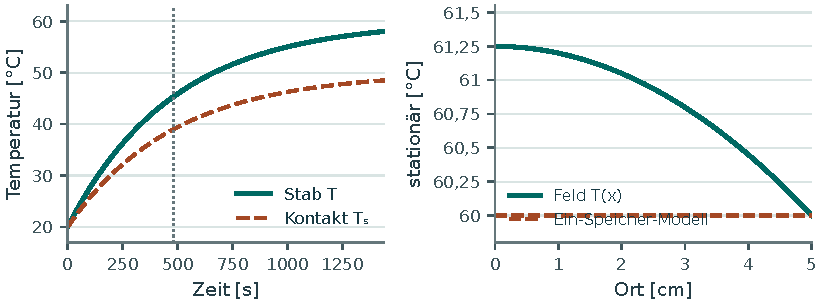
\includegraphics[width=.88\linewidth,height=49mm,keepaspectratio]{thermisch.pdf}\par}\capline{Temperatur, gespeicherte Energie und momentane Leistung bezeichnen drei verschiedene Größen.}
\seite{}{Dynamische Systeme und Steifigkeit}\anchorpage{2}{abs1-1}{1.1 · Kontinuierliche Systeme im Zustandsraum}\ey{ABSCHNITT 1.1}\ptitle{Kontinuierliche Systeme im Zustandsraum}
\hypertarget{punkt1-1-1}{}\subt{1.1.1\enspace Vektorfelder, Phasenporträts und Trajektorien}
Ein Wagen passiert zweimal dieselbe Markierung. Einmal fährt er zum Anschlag, einmal zurück. Erst der Punkt \(y=(q,v)\) unterscheidet beide Situationen. Beim Federwagen mit Masse \(m\), Federkonstante \(k\) und Dämpfung \(d\) zeigt der Pfeil an diesem Punkt in Richtung \((v,-(kq+dv)/m)\). Die Gesamtheit dieser Pfeile heißt Vektorfeld. Eine Trajektorie folgt den Pfeilen ab einem gewählten Start. Im Phasenporträt liegt die Auslenkung auf der waagerechten, die Geschwindigkeit auf der senkrechten Achse. Bei positiver Auslenkung und Geschwindigkeit null zeigt der Pfeil abwärts.
\hypertarget{punkt1-1-2}{}\subt{1.1.2\enspace Autonome Systeme und die Zeit als Zustand}
Wird der Wagen von außen mit \(F_0\cos(\omega t)\) angeregt, können am gleichen Punkt zu zwei Zeiten verschiedene Pfeile stehen. Ergänzen wir die Uhr \(s'=1,\ s(0)=t_0\), wird das erweiterte Feld \((s',q',v')=(1,v,(F_0\cos(\omega s)-kq-dv)/m)\) autonom. Die zusätzliche Koordinate trägt die Phase der Anregung.
\hypertarget{punkt1-1-3}{}\subt{1.1.3\enspace Bilanzen, Erhaltungsgrößen und Hamilton-Systeme}
Mit Impuls \(p=mv\) und Energie \(H=p^2/(2m)+kq^2/2\) gelten ohne Antrieb und Reibung \(q'=H_p,\ p'=-H_q\). Die Kettenregel ergibt \(H'=H_qH_p-H_pH_q=0\). Die geschlossenen Ellipsen im Phasenporträt sind Energieniveaus. Reibung ergänzt \(-dv\) in der Impulsbilanz und liefert \(H'=-dv^2\). Eine nach außen wandernde Rechnung kann dann bereits durch das Vorzeichen der Energiebilanz widerlegt werden.
\seite{Rechenbeispiel}{Dynamische Systeme und Steifigkeit}\anchorpage{2}{kap1}{Welche Information fehlt dem Messgerät?}\ptitle{Welche Information fehlt dem Messgerät?}


\lernziel{Sie können aus zwei Beobachtungen einen Zustand bestimmen und angeben, welche äußere Größe für eine Vorhersage noch fehlt.}
Ein Vorratsbehälter hat laut Anzeige genau 12 Liter Inhalt. In fünf Sekunden soll ein Ventil öffnen, falls dann mindestens 14 Liter bereitstehen. Können Sie das Ventil schon jetzt freigeben? Zeichnen Sie zwei mögliche Füllkurven durch denselben angezeigten Punkt.
\subt{Was wir über den Behälter annehmen}
Im betrachteten Zeitfenster läuft er weder über noch leer. Zufluss und Abfluss seien je Versuch konstant. Ein Durchflussmesser zeigt in Versuch A einen Nettozufluss von \(0{,}6\unitm{L/s}\), in Versuch B sind es \(0{,}2\unitm{L/s}\). Das Vorzeichen „plus“ bedeutet, dass Wasser im Behälter hinzukommt.
\subt{Eine Vorhersage für jeden Versuch}
In A kommen \(5\cdot0{,}6=3\unitm L\) hinzu. Der Behälter erreicht \(15\unitm L\). In B kommt nur ein Liter hinzu. Mit \(13\unitm L\) bleibt das Ventil zu. Die Zahl auf der Anzeige war in beiden Fällen richtig. Die Zukunft hing zusätzlich davon ab, was während der fünf Sekunden von außen zugeführt wurde.
\notebox{Jetzt Sie}{Die Anzeige bleibt bei \(12\unitm L\). Welcher konstante Nettozufluss reicht gerade? Schreiben Sie erst einen Bruch mit Einheiten. Die Kontrolle lautet \( (14-12)\unitm L/(5\unitm s)=0{,}4\unitm{L/s}\). Bei genau diesem Wert öffnet das Ventil.}
Beim Wagen führt dieselbe Frage zu einer anderen fehlenden Information. Selbst wenn alle künftigen Kräfte bekannt sind, genügt die aktuelle Position allein noch nicht.

\srcs{\textbf{Kernweg}\enspace\see{grund}{Zustand des Wagens}\quad\textbf{Vertiefung}\enspace\see{periodenformel}{Exakte Pendelperiode}\quad\see{ueb1}{Selbst prüfen}.}

\lektion{Wie viel Gegenwart braucht eine Vorhersage?}{grund}{Kernweg}{Dynamische Systeme}
\vorhersage{1}{Zwei Pumpen haben zu Beginn und am Ende einer Sekunde dieselben Förderraten. Liefern sie gleich viel Wasser?}{kontrolleA}
Eine Lichtschranke zählt einen Wagen bei \(q=1\unitm m\). Die Strecke ist horizontal und der Wagen rollt eine Sekunde lang kräftefrei. Zeichnen Sie zwei Pfeile durch denselben Ort. Mit \(v=+0{,}5\unitm{m/s}\) liegt der Wagen danach bei \(1{,}5\unitm m\), mit \(v=-0{,}5\unitm{m/s}\) bei \(0{,}5\unitm m\). Welche zweite Angabe fehlt der Lichtschranke?
\minifig{zustaende}{42mm}{Links laufen beide Bahnen durch denselben Messpunkt. Rechts unterscheidet die zweite Koordinate, die Geschwindigkeit, die beiden Bewegungen.}
\subt{System, Zustand, Eingang, Ausgang}
Ein \emph{System} ist der abgegrenzte Gegenstand unserer Beschreibung. Sein \emph{Zustand} fasst für die betrachtete Aufgabe alle Informationen zusammen, die bei bekanntem künftigen Eingang die weitere Entwicklung bestimmen. Der \emph{Eingang} kann von außen vorgegeben werden, etwa die Zugkraft. Der \emph{Ausgang} ist die beobachtete Größe, etwa die Lichtschrankenposition. Eine zeitliche Folge von Zuständen heißt \emph{Trajektorie}.

Für den kraftfreien Wagen genügt das Paar \((q,v)\). Auch eine einzelne Masse auf einer Feder lässt sich so beschreiben. Eine zweite bewegliche Masse könnte zusätzliche Zustände erfordern.
\notebox{Selbstkontrolle}{Ein Tank enthält 20 Liter. Kennen wir den konstanten Querschnitt und alle Zu- und Abflüsse bis in zehn Sekunden, können wir den künftigen Pegel berechnen. Bei unbekannter Ventilstellung fehlt ein Eingang.}

\lektion{Von zwei Messpunkten zur Bilanz}{ableitung}{Kernweg}{Dynamische Systeme}
Der Wagen passiert bei \(t=0\unitm s\) und \(t=2\unitm s\) die Marken \(q=1\unitm m\) und \(q=2\unitm m\). Die mittlere Geschwindigkeit im Intervall ist \( (2-1)/(2-0)=0{,}5\unitm{m/s}\). Bei veränderlicher Geschwindigkeit interessiert die Steigung der Ortskurve genau jetzt. Für einen glatten Verlauf definieren wir
\[
 v(t)=\dot q(t)=q'(t)=\lim_{h\to0}\frac{q(t+h)-q(t)}{h}.
\]
Ein Punkt bedeutet zeitliche Ableitung. Der zweite Punkt \(\ddot q=\dot v\) bedeutet Beschleunigung. Für \(q(t)=q_0+v_0t+at^2/2\) ergibt der Differenzenquotient \(v_0+at+ah/2\). Sein Grenzwert ist \(v_0+at\). Die Einheit wechselt bei jeder Zeitableitung um einen Faktor \(\mathrm{s}^{-1}\).
\subt{Rückwärts denken führt zum Integral}
In einem kurzen Intervall \(\Delta t_i\) legt der Wagen ungefähr \(v(t_i)\Delta t_i\) zurück. Addiert man diese Beiträge und lässt die größte Intervalllänge gegen null gehen, entsteht für stetiges \(v\) das bestimmte Integral
\[
 q(b)-q(a)=\int_a^b v(t)\dg t.
\]
Bei \(v(t)=2t\unitm{m/s}\) für den Zahlenwert \(t\) in Sekunden ergibt die Dreiecksfläche von 0 bis 3 Sekunden \(9\unitm m\). Differenzieren und Integrieren verbinden eine momentane Rate mit der Änderung im ganzen Zeitintervall. Das ist die Grundlage jeder Speicherbilanz.
\subt{Eine Gleichung aus Worten gewinnen}
Ein Tank erhält \(3\unitm{L/s}\) und gibt \(1\unitm{L/s}\) ab. In fünf Sekunden wächst sein Inhalt um \(10\unitm L\). In Symbolen lautet die Bilanz \(\dot V=Q_\mathrm{ein}-Q_\mathrm{aus}\). Diese Gleichung bestimmt die Änderung. Erst die zusätzliche Angabe \(V(0)=20\unitm L\) legt den Inhalt nach fünf Sekunden auf \(30\unitm L\) fest. Eine Funktion zusammen mit ihren geforderten Anfangsdaten zu bestimmen heißt, ein \emph{Anfangswertproblem} zu lösen.
\notebox{Einheitenprobe}{In einer Summe müssen alle Summanden dieselbe physikalische Dimension haben. Im Tank steht auf beiden Seiten Volumen pro Zeit. Eine Formel \(\dot V=Q_\mathrm{ein}-V\) braucht vor \(V\) einen Faktor mit der Einheit \(1/\mathrm s\).}

\lektion{Braucht diese Aufgabe einen Zeitschritt?}{methodenwahl}{Kernweg}{Dynamische Systeme}
Ein Tank enthält 20 Liter. Pro Sekunde fließen drei Liter hinein und einer hinaus. Wie viel Wasser ist nach fünf Sekunden im Tank? Bei konstanten Raten gilt bis zum Überlauf für die Zeit \(t\) in Sekunden
\[
 V(t)=(20+2t)\unitm L .
\]
Nach fünf Sekunden sind es \(30\unitm L\). Umgekehrt folgt aus \(20+2t=40\), dass die 40-Liter-Marke nach zehn Sekunden erreicht ist.
\subt{Was ändert sich bei einem geregelten Ventil?}
Nun misst ein Sensor den Zufluss. Der Abfluss hängt vom Wasserstand ab. Bei einem Grenzstand schaltet der Regler das Ventil. Für jeden Schritt berechnen wir aus den Flüssen den neuen Stand und daraus den nächsten Abfluss. Überschreitet der Stand die Schwelle, suchen wir die Schaltzeit innerhalb des Schritts. Dafür müssen wir auch festlegen, wie wir den Zufluss zwischen zwei Messwerten annähern.
\subt{Zwei Entscheidungen vor der Rechnung}
{\tblstart\begin{tabularx}{\linewidth}{@{}P{30mm}YY@{}}\toprule
\hd{Modell}&\hd{Analytisch lösen}&\hd{Numerisch lösen}\\\midrule
Ursprüngliche Gleichungen&Formel, Erhaltungssatz oder Integral für die gesuchte Größe herleiten.&Aus dem gegebenen Gesetz einzelne Werte oder eine ganze Bahn berechnen.\\
Am Arbeitspunkt linearisiertes Modell&Eine Formel beschreibt die Reaktion auf kleine Störungen.&Die linearen Gleichungen etwa mit einem aufgezeichneten, zeitlich wechselnden Eingang integrieren.\\\bottomrule\end{tabularx}\par}
Gekoppelte Gleichungen, gemessene Eingänge und viele Schaltvorgänge erschweren eine geschlossene Lösung. Auch ein lineares Wärmemodell mit tausend Temperaturen lässt sich sinnvoll numerisch auswerten.
\notebox{Entscheidung für den Versuch}{Den Füllstand bei konstanten Raten liefert die Formel. Für kleine Schwankungen um einen stationären Stand prüfen wir die Linearisierung. Für die erste Schaltzeit brauchen wir den gemessenen Zufluss, die Schaltregel und eine geforderte Zeitgenauigkeit.}
\srcs{\see{arbeitspunkt}{Arbeitspunkt und Tangente} · \see{periodentest}{Ein Fehlerziel am Pendel} · \see{c07modell}{Ereigniszeiten im ARGESIM-Versuch}.}

\lektion{Vektoren, Matrizen und ein Maß für Fehler}{vektor}{Kernweg}{Dynamische Systeme}
Ein \emph{Skalar} ist eine einzelne Zahl. Ein \emph{Vektor} fasst mehrere geordnete Zahlen zu einem Objekt zusammen. Für den Wagen schreiben wir \(x=(q,v)^\mathsf T\) als Spalte. \({}^\mathsf T\) vertauscht Zeile und Spalte. \(\mathbb R^n\) bezeichnet alle Spalten mit \(n\) reellen Einträgen. Verschiedene Einträge dürfen verschiedene Einheiten haben.
\subt{Eine Matrix als Rechenvorschrift}
Eine Matrix bildet durch Zeile-mal-Spalte einen Vektor auf einen anderen ab. Beim kraftfreien Wagen ergibt die exakte Fortrechnung über \(h\) Sekunden
\[
 \begin{pmatrix}q(t+h)\\v(t+h)\end{pmatrix}
 =\underbrace{\begin{pmatrix}1&h\\0&1\end{pmatrix}}_{A(h)}
 \begin{pmatrix}q(t)\\v(t)\end{pmatrix}.
\]
Die erste Zeile addiert den in \(h\) Sekunden zurückgelegten Weg. Die zweite übernimmt die Geschwindigkeit. Zwei Schritte \(h,k\) ergeben durch Matrixmultiplikation \(A(k)A(h)=A(h+k)\). Die Einheitsmatrix \(I=A(0)\) lässt jeden Vektor unverändert.
\subt{Lösbar und eindeutig}
Eine quadratische Matrix ist \emph{invertierbar}, wenn jede rechte Seite \(b\) in \(Ax=b\) genau eine Lösung besitzt. Bei zwei Zeilen und zwei Spalten entscheidet die Determinante \(ad-bc\) für \(A=\left(\begin{smallmatrix}a&b\\c&d\end{smallmatrix}\right)\). Sie muss ungleich null sein. Der \emph{Rang} zählt linear unabhängige Spalten, äquivalent die unabhängigen Zeilen. Zwei gleiche Messzeilen liefern nur eine unabhängige Information.
\subt{Wie groß ist ein Vektor?}
Eine Norm ordnet einem Vektor eine nichtnegative Länge zu. Die Maximumnorm ist \(\|z\|_\infty=\max_i |z_i|\), die euklidische Norm \(\|z\|_2=\sqrt{\sum_i z_i^2}\). Vor einem Zahlenvergleich zwischen Ort und Geschwindigkeit teilen wir jeden Fehler durch seine zulässige Abweichung. Bei Fehlern \(2\unitm{mm}\), \(0{,}03\unitm{m/s}\) und Grenzen \(5\unitm{mm}\), \(0{,}02\unitm{m/s}\) entsteht \(z=(0{,}4,1{,}5)^\mathsf T\). Die Maximumnorm \(1{,}5\) zeigt sofort, welche Komponente durchfällt.
\srcs{Mit demselben Gedanken bewertet das Praktikum mehrere Ereigniszeiten und Endwerte auf S.\,\pagelink{vergleich}.}

\lektion{Wie Mathematik eine Näherung beschreibt}{mathewerk}{Vertiefung}{Dynamische Systeme}
Für eine kleine Änderung \(h\) liefert die Tangente \(f(x+h)\approx f(x)+hf'(x)\). Die \emph{Taylorformel} gibt bei zweimal stetig differenzierbarem \(f\) den Rest als \(h^2 f''(\xi)/2\) an, mit \(\xi\) zwischen \(x\) und \(x+h\). Die Schreibweise \(O(h^p)\) bedeutet, dass der Betrag für hinreichend kleine \(|h|\) höchstens \(C|h|^p\) beträgt, mit einer von \(h\) unabhängigen Konstanten \(C\).
\subt{Exponent, Logarithmus und eine Zeitkonstante}
Die Exponentialfunktion \(e^z=\sum_{k=0}^\infty z^k/k!\) ist ihre eigene Ableitung. Deshalb löst \(x(t)=x_0e^{-t/\tau}\) die Gleichung \(\dot x=-x/\tau\) für \(\tau>0\). Nach einer Zeitkonstante bleibt der Anteil \(1/e\). Der natürliche Logarithmus \(\ln\) ist die Umkehrfunktion von \(e^z\) für positive reelle Argumente. Die Halbwertszeit folgt aus \(e^{-t/\tau}=1/2\), also \(t=\tau\ln 2\).
\subt{Eine Änderung in mehreren Richtungen}
Hängt \(f\) von \(x\) und \(z\) ab, variiert die partielle Ableitung \(f_x=\partial f/\partial x\) nur \(x\) bei festem \(z\). Für \(f(x,z)=xz^2\) sind \(f_x=z^2\) und \(f_z=2xz\). Entlang einer Bahn gilt die Kettenregel
\[
 \frac{\dd}{\dd t}f(x(t),z(t))=f_x\dot x+f_z\dot z .
\]
Hat die Funktion mehrere Ausgaben \(f_i\), sammelt die \emph{Jacobi-Matrix} die partiellen Ableitungen in \(J_{ij}=\partial f_i/\partial x_j\). Sie ist die lokale lineare Abbildung \(f(x+\delta x)\approx f(x)+J(x)\delta x\). Hat \(f\) zusätzlich eine ausdrückliche Zeitabhängigkeit, kommt in der Kettenregel \(f_t\) hinzu.
\subt{Wie löst man eine Gleichung, die sich nicht umstellen lässt?}
Ein \emph{Residuum} \(r(z)\) misst die Verletzung einer Gleichung. Gesucht ist eine Nullstelle. Newton löst \(r'(z_k)\Delta z=-r(z_k)\) und setzt \(z_{k+1}=z_k+\Delta z\). Für \(r=z^2-2,\ z_0=1{,}5\) folgt \(z_1=1{,}41667\). Das Verfahren braucht lokal eine brauchbare Steigung. Bei stetigem \(r\) und entgegengesetzten Vorzeichen an den Enden kann Intervallhalbierung dagegen eine Nullstelle einklammern. Ein bloßer Berührpunkt hat nicht zwingend einen Vorzeichenwechsel.

\seite{Rechenbeispiel}{Dynamische Systeme und Steifigkeit}\anchorpage{2}{kap3}{Was verraten zwei Heizversuche?}\ptitle{Was verraten zwei Heizversuche?}


\lernziel{Sie können eine Systemgrenze ziehen, gespeicherte Energie und Leistung unterscheiden und aus zwei Versuchen erkennen, welche Modellparameter messbar sind.}
Ein Heizer führt einem Metallstück \(10\unitm W\) zu. Eine Minute später ist es wärmer. Reicht diese Beobachtung, um vorherzusagen, wie heiß es im Dauerbetrieb wird? Zeichnen Sie einen Rahmen um das Metall und geben Sie jedem Energiestrom einen Pfeil.
\subt{Erst die Bilanz, dann das Bauteilgesetz}
Wir nehmen eine überall gleiche Metalltemperatur an. Seine Wärmekapazität \(C=120\unitm{J/K}\) sagt, wie viel Energie einen Temperaturanstieg um ein Kelvin bewirkt. Am Start haben Metall und Umgebung dieselbe Temperatur. Im ersten Augenblick fließt daher noch keine Wärme an die Umgebung. Die gesamte Leistung erhöht die gespeicherte Energie. Die Anfangssteigung ist \(10/120=0{,}0833\unitm{K/s}\).
\subt{Ein zweiter Versuch beantwortet eine andere Frage}
Lange nach dem Einschalten beträgt der Überschuss zur Umgebung konstant \(40\unitm K\). Jetzt muss der Abfluss die ganzen \(10\unitm W\) übernehmen. Im linearen Kontaktgesetz \(\theta=Rq\) ergibt das einen Wärmewiderstand \(R=40/10=4\unitm{K/W}\). Die Anfangssteigung lieferte \(C\), der stationäre Versuch liefert \(R\).
\notebox{Jetzt Sie}{Eine zweite Halterung halbiert \(R\) bei gleichem \(C\) und gleicher Heizleistung. Skizzieren Sie beide Aufheizkurven mit gemeinsamen Sekunden- und Kelvinachsen. Beide starten mit derselben Steigung. Die neue Kurve läuft auf \(20\unitm K\) Überschuss zu.}
Das Kapitel verwendet denselben Heizer für drei Fragen. Wie warm wird das ganze Stück? Welche Temperatur hat der Kontakt? Und wo liegt im Innern der heißeste Punkt? Jede Messfrage verlangt andere Zustandsgrößen.

\srcs{\textbf{Kernweg}\enspace\see{speicher}{Bilanz und Temperatur}\quad\textbf{Vertiefung}\enspace\see{moden}{Beobachtbarkeit}\quad\see{ueb3}{Selbst prüfen}.}

\lektion{Ein Stab, ein Heizer und zwei Kontakte}{modell}{Kernweg}{Modell und System}
\vorhersage{3}{Ein Heizer liefert konstante Leistung. Welchen Einfluss hat die doppelte Wärmekapazität auf Endtemperatur und Aufheizzeit?}{kontrolleA}
Eine Halterung führt Wärme von einem beheizten Metallstab ab. Gesucht sind die Aufwärmzeit, die höchste Dauertemperatur und die Temperatur im Kontakt. Der Heizer liefert \(10\unitm W\), die Umgebung bleibt bei \(20\,^\circ\mathrm C\), Mantel und linke Stirnfläche sind isoliert. Verfolgen Sie den Weg der Energie erst in der Skizze.
\fig{stab}{.90}{Ein positiver Wärmestrom \(q=\dot Q\) verlässt den Stab nach rechts. Zwischen den Kontaktwiderständen liegt die Temperatur \(T_s\).}
\subt{Welche Daten gehören zur Bilanz?}
{\tblstart\begin{tabularx}{\linewidth}{@{}P{47mm}rY@{}}\toprule
\hd{Größe} & \hd{Wert} & \hd{Bedeutung}\\\midrule
Länge \(L\), Querschnitt \(A\)& \(0{,}05\unitm m,\;10^{-3}\unitm{m^2}\)& konstanter Querschnitt\\
Volumetrische Wärmekapazität \(\rho c\)& \(2{,}4\cdot10^6\)& \(\mathrm{J/(m^3 K)}\)\\
Wärmeleitfähigkeit \(k\)& \(200\unitm{W/(m\,K)}\)& homogener Werkstoff\\
Widerstände \(R_1,R_2\)& \(1,\;3\unitm{K/W}\)& in Reihe zum Reservoir\\\bottomrule
\end{tabularx}\par}
Die Leistung \(P\) sei gleichmäßig im Volumen verteilt. Der Stab startet bei \(20\,^\circ\mathrm C\). Stoffwerte und Querschnitt bleiben konstant, beide Kontaktlagen speichern vernachlässigbar wenig Wärme. Eine sich erwärmende Umgebung wäre ein weiterer Speicher.
\subt{Erster Überschlag vor der Integration}
Der Stab speichert \(C=\rho cAL=120\unitm{J/K}\). Gleich nach dem Einschalten fließt am kalten Kontakt noch keine Leistung ab. Damit steigt die mittlere Temperatur anfangs um \(P/C=1/12\unitm{K/s}\). Im Dauerbetrieb muss dieselbe Leistung, die eintritt, über die Halterung austreten. Diese zwei Werte prüfen später jede Simulation.
\srcs{Annahmen, Geometrie und Zahlenwerte sind Lehrbeispieldaten.}

\lektion{Aus der Energiebilanz folgt eine ODE}{speicher}{Kernweg}{Modell und System}
Wir ersetzen die Temperaturverteilung vorläufig durch eine einzige Temperatur \(T(t)\). Mit \(\theta=T-T_a\) in Kelvin und \(R=R_1+R_2=4\unitm{K/W}\) folgt aus dem Energieinhalt \(C\theta\) und dem Ausfluss \(q=\theta/R\)
\[
 C\dot\theta=P-\frac{\theta}{R},\qquad \theta(0)=0.
\]
Links steht die Änderungsrate \(\dot E=C\dot\theta\) der gespeicherten Energie \(E=C\theta\). Alle Terme der Bilanz haben die Einheit Watt. Nach Wahl von \(P(t)\) und \(\theta(0)\) ist die Ableitung bestimmt. Das ist ein Anfangswertproblem für eine gewöhnliche Differentialgleichung (ODE).
\subt{Die Rechnung für einen Leistungssprung}
Im Gleichgewicht gilt \(\theta_\infty=RP=40\unitm K\). Für \(w=\theta-\theta_\infty\) bleibt \(\dot w=-w/(RC)\). Trennung der Variablen liefert
\[
 \theta(t)=40(1-e^{-t/480})\unitm K,\qquad \tau=RC=480\unitm s
\]
mit \(t\) in Sekunden. Nach \(60\unitm s\) liegen \(24{,}700124\,^\circ\mathrm C\) vor. Der Stab hat relativ zum Start \(C\theta=564{,}015\unitm J\) gespeichert. In diesem Moment steigt seine Energie mit \(10\unitm W-\theta/R=8{,}82497\unitm W\). Nach \(\tau\) sind \(1-e^{-1}=63{,}2\,\%\) des Temperaturanstiegs erreicht. Der Kontakt folgt aus \(T_s=T_a+R_2q\). Im stationären Zustand ergibt das \(50\,^\circ\mathrm C\).
\fig{thermisch}{.96}{Links folgt der Kontakt dem Stab mit kleinerem Temperaturhub. Rechts zeigt das räumliche Modell unter denselben Randbedingungen, wo ein Ein-Speicher-Modell die Höchsttemperatur unterschätzt.}
\notebox{Reicht ein Speicher?}{Der innere Leitwiderstand hat die Skala \(L/(kA)=0{,}25\unitm{K/W}\). Das Verhältnis zur äußeren Reihenschaltung beträgt \(0{,}0625\). Der räumliche Temperaturabfall kann für die Aufwärmzeit klein und für einen Grenzwert von nur \(0{,}5\unitm K\) dennoch entscheidend sein.}
\srcs{Die stationäre Feldlösung wird auf S.\,\pagelink{pde} aus denselben Stoffdaten hergeleitet.}

\lektion{ODE, DAE und PDE am selben Gegenstand}{klassen}{Kernweg}{Modell und System}
Nehmen Sie denselben Stab. Zuerst interessiert nur eine gut durchmischte Temperatur. Dann wollen wir den Wärmestrom am Kontakt direkt ausgeben. Zuletzt fragen wir nach der heißesten Stelle im Stab. Die Physik bleibt wiedererkennbar, aber jede Aufgabenstellung braucht andere Unbekannte.
{\tblstart\begin{tabularx}{\linewidth}{@{}P{17mm}YY@{}}\toprule
\hd{Form}&\hd{Unbekannte und Gleichung}&\hd{Physikalische Aussage}\\\midrule
ODE&\(\theta(t)\), \(\ C\dot\theta=P-\theta/R\)&Ein Wärmespeicher. Der Wärmestrom ist bereits eliminiert.\\
DAE&\(\theta(t),\,\theta_s(t),\,q(t)\), \(\ C\dot\theta=P-q\) mit zwei Kontaktgesetzen&Ein Wärmespeicher und zwei augenblickliche Beziehungen.\\
PDE&\(T(x,t)\), \(\ \rho c A\,T_t=kA\,T_{xx}+P/L\)&Jedes Stabstück speichert Wärme. Ort, Randwerte und Anfangsprofil werden gebraucht.\\\bottomrule
\end{tabularx}\par}
\subt{Zwei verschiedene Entscheidungen}
\textbf{Algebraische Elimination.} Aus \(\theta-\theta_s=R_1q\) und \(\theta_s=R_2q\) folgt exakt \(q=\theta/(R_1+R_2)\). Damit sind ODE und DAE für die Stabtemperatur bei konsistenten Daten gleichwertig. Eine eigene Wärmekapazität des Kontakts würde das Modell verändern.

\textbf{Räumliche Mittelung.} Die exakte Integralbilanz lautet \(C\dot{\bar T}=P-q(L,t)\), wobei \(\bar T=L^{-1}\int_0^L T(x,t)\dg x\). Der Randstrom hängt von \(T(L,t)\) ab. Erst die Annahme \(T(L,t)\approx\bar T(t)\) schließt die Gleichung für einen einzigen Speicher. Hier entsteht ein Modellfehler.
\subt{Wie passen PDE und DAE zusammen?}
Die PDE kann am Rand mit einer algebraischen Kontaktgleichung gekoppelt sein. Diskretisiert man den Ort, erhält man Differentialgleichungen für Zelltemperaturen. Ein beibehaltener masseloser Kontakt fügt algebraische Gleichungen hinzu. Nach Elimination dieses Kontakts bleibt in diesem Beispiel eine ODE für die Zelltemperaturen.
\task{1}{Für einen thermisch trägen Kontakt mit Wärmekapazität \(C_s>0\) treten links \(q_1\) ein und rechts \(q_2\) aus. Stellen Sie das Zweitemperaturmodell auf. Welche Gleichung entsteht im Grenzmodell \(C_s=0\)?}

\lektion{Was ein Zustand über die Zukunft verrät}{system}{Kernweg}{Modell und System}
Was müssen Sie beim Speichern einer laufenden Simulation sichern, damit ein Neustart dieselbe Zukunft erzeugt? Beim ideal durchmischten Stab genügt die Temperatur, wenn die zukünftige Heizleistung bekannt ist. Bei einer fallenden Kugel gehört auch die Geschwindigkeit dazu. Von gleicher Höhe kann eine Kugel gerade steigen und die andere fallen.
\subt{Eingang, Zustand und Ausgang}
Im Modell \(\dot x=f(x,u,t),\ y=h(x,u,t)\) bezeichnet \(u\) die von außen vorgegebene Anregung und \(y\) die Messgröße. Für ein lineares, zeitinvariantes System (LTI) mit konstanten Matrizen gilt
\[
 \dot x=A_sx+B_su,\qquad y=C_s^{\rm out}x+D_s u .
\]
Die Indizes unterscheiden Systemmatrizen von Fläche und Wärmekapazität. Beim Stab mit \(u=P,\ x=\theta,\ y=\theta\) sind \(A_s=-1/(RC),\ B_s=1/C,\ C_s^{\rm out}=1,\ D_s=0\).
\subt{Zeitantwort und Frequenzantwort aus derselben Gleichung}
Variation der Konstanten ergibt
\[
 x(t)=e^{A_st}x(0)+\int_0^t e^{A_s(t-s)} B_su(s)\dg s .
\]
Zur Kontrolle differenziert man die rechte Seite. Die obere Integrationsgrenze liefert \(B_su(t)\), die übrigen Terme ergeben \(A_sx(t)\). Bei Anfangswert null folgt durch Laplace-Transformation die Übertragungsfunktion
\[
 G(s)=C_s^{\rm out}(sI-A_s)^{-1}B_s+D_s=\frac{R}{1+sRC}
 \quad\text{für den Stab.}
\]
Im stationären Sinusbetrieb ist der Verstärkungsbetrag \(R/\sqrt{1+(\omega\tau)^2}\), die Phase \(-\arctan(\omega\tau)\). Bei \(\omega=1/\tau\) bedeuten \(1\unitm W\) Eingangsamplitude \(4/\sqrt 2=2{,}83\unitm K\) Ausgangsamplitude und \(45^\circ\) Nacheilen. Der Pol \(-1/\tau\) bestimmt also Aufwärmzeit und Grenzfrequenz zugleich.
\srcs{\refbk{sy}{Åström und Murray, Feedback Systems} · Zustand, lineare Dynamik und Eingangs-/Ausgangsbeschreibung.}

\lektion{Vom Rechnen mit Matrizen zur Systemtheorie}{linearsprache}{Kernweg}{Modell und System}
Eine Abbildung \(A\) heißt \emph{linear}, wenn \(A(\alpha x+\beta z)=\alpha A x+\beta A z\). Damit lassen sich Antworten auf einzelne Anregungen addieren. \emph{Zeitinvariant} bedeutet, dass eine Verschiebung des gesamten Versuchs in der Zeit dasselbe Verhalten mitverschiebt. Ein System mit konstanten Matrizen ist ein wichtiges Beispiel.
\subt{Warum Eigenwerte in einer Zeitentwicklung auftauchen}
Erfüllt ein Vektor \(w\ne0\) die Gleichung \(Aw=\lambda w\), heißt \(w\) Eigenvektor und \(\lambda\) Eigenwert. Für \(\dot x=Ax\) löst dann \(x=e^{\lambda t}w\) die Differentialgleichung, wie Ableiten zeigt. Ein solcher Bewegungsanteil heißt \emph{Mode}. Das Matrixexponential \(e^{At}=I+At+(At)^2/2!+\cdots\) fasst die Fortrechnung für alle Anfangsvektoren zusammen.

Komplexe Zahlen \(s=\sigma+\mathrm i\omega\) verwenden \(\mathrm i^2=-1\). Wegen \(e^{st}=e^{\sigma t}(\cos\omega t+\mathrm i\sin\omega t)\) beschreibt \(\sigma\) Wachstum oder Abklingen und \(\omega\) eine Kreisfrequenz in Radiant pro Sekunde. Ein Radiant ist der Winkel, dessen Bogenlänge auf einem Kreis gleich dem Radius ist. Eine volle Umdrehung entspricht \(2\pi\) Radiant. Die reale Messgröße kann einfach der Realteil sein.
\subt{Ein Werkzeug für Eingangs- und Ausgangsgrößen}
Die Laplace-Transformierte eines Signals \(w(t)\) ist \(W(s)=\int_0^\infty e^{-st}w(t)\dg t\), wo das Integral konvergiert. Partielle Integration liefert \(\mathcal L\{\dot w\}=sW(s)-w(0)\). Eine Differentialgleichung wird so zur algebraischen Beziehung in \(s\).

Beim Stab ergibt \(C\dot\theta+\theta/R=P\) bei kaltem Start \((Cs+1/R)\Theta(s)=P(s)\). Der Quotient \(G(s)=\Theta(s)/P(s)\) heißt \emph{Übertragungsfunktion}. Ein \emph{Pol} ist hier eine Nullstelle des Nenners, an der der Quotient unbeschränkt wird. Die Position \(-1/(RC)\) ist dieselbe Abklingrate, die die Zeitlösung enthält. Für stabilen eingeschwungenen Sinusbetrieb setzt man \(s=\mathrm i\omega\).
\srcs{\refbk{sy}{Åström und Murray, Zustandsraum und Frequenzantwort} · \see{arbeitspunkt}{Wie aus einem nichtlinearen System ein lokales lineares Modell wird}.}

\lektion{Was bedeutet Linearisieren im Arbeitspunkt?}{arbeitspunkt}{Kernweg}{Dynamische Systeme}
Ein Pendel hängt senkrecht und ruht. Eine kleine Auslenkung erzeugt eine rücktreibende Beschleunigung. Für einen Entwurf nahe dieser Lage interessiert zunächst, wie sich die Beschleunigung bei einer kleinen Störung ändert. Dafür genügt häufig die Tangente an das Bewegungsgesetz.
\subt{Vom Arbeitspunkt zur Gleichung für kleine Abweichungen}
Bei einem zeitunabhängigen Gesetz \(\dot x=f(x,u)\) ist ein \emph{stationärer Arbeitspunkt} ein Paar aus Zustand \(x_*\) und konstantem Eingang \(u_*\) mit \(f(x_*,u_*)=0\). Für \(\delta x=x-x_*,\ \delta u=u-u_*\) liefert die Taylorformel
\[
 \delta\dot x=A\,\delta x+B\,\delta u+r,\qquad
 A=\left.\frac{\partial f}{\partial x}\right|_*,\quad
 B=\left.\frac{\partial f}{\partial u}\right|_* .
\]
Die Matrizen geben an, wie sich jede Steigung mit Zustand und Eingang ändert. Bei zweimal stetig differenzierbarem \(f\) ist der Rest nach geeigneter Skalierung lokal von der Größenordnung \(\|(\delta x,\delta u)\|^2\). Das lineare Modell setzt \(r=0\). Es eignet sich beispielsweise für die Frequenz kleiner Schwingungen oder die Auslegung eines Reglers nahe seinem Sollwert.
\subt{Am Pendel lässt sich die Tangente ausrechnen}
Seien \(L\) die Länge, \(g\) die Fallbeschleunigung und \(u\) eine von außen aufgeprägte Winkelbeschleunigung. Mit \(\theta\) als Winkel zur unteren Senkrechten, in Radiant, und \(\omega=\dot\theta\) gilt ohne Reibung
\[
 \dot\theta=\omega,\qquad \dot\omega=-(g/L)\sin\theta+u .
\]
Am Arbeitspunkt \((\theta_*,\omega_*,u_*)=(0,0,0)\) ist die Steigung des Sinus gleich eins. Bei \(u=0\), Startwinkel \(\theta_0\) und Startgeschwindigkeit null führt \(\sin\theta\approx\theta\) zu
\[
 \theta_{\rm lin}(t)=\theta_0\cos\!\big(\sqrt{g/L}\,t\big),\qquad
 T_0=2\pi\sqrt{L/g}.
\]
Einsetzen bestätigt diese Lösung des linearen Modells. Dessen Periodendauer \(T_0\) ist für jede von null verschiedene Amplitude gleich. Beim ursprünglichen Pendel hängt die Dauer von der Amplitude ab. Wie groß der Unterschied ist, können wir ohne Messgerät herleiten.
\srcs{\href{https://underactuated.mit.edu/acrobot.html}{Tedrake, Linearisierung an einem Fixpunkt} · \href{https://openstax.org/books/university-physics-volume-1/pages/15-4-pendulums}{OpenStax, Pendel und Kleinwinkelnäherung}.}

\lektion{Welche Mode sieht der Sensor?}{moden}{Vertiefung}{Modell und System}
Zwei gleiche Metallblöcke haben je \(C_b=60\unitm{J/K}\). Jeder gibt über \(G_e=0{,}125\unitm{W/K}\) Wärme an dieselbe Umgebung ab. Zwischen beiden fließen \(G_c(\theta_1-\theta_2)\) Watt mit \(G_c=2\unitm{W/K}\). Ein Heizer wirkt nur am ersten Block. Die Kontaktleistung tritt mit entgegengesetztem Vorzeichen in die beiden Bilanzen ein.
\[
 \dot x=\begin{bmatrix}-(a+b)&b\\ b&-(a+b)\end{bmatrix}x+
 \begin{bmatrix}1/C_b\\0\end{bmatrix}P,\qquad
 a=G_e/C_b,\quad b=G_c/C_b .
\]
Addiert man die Bilanzen, verschwindet der innere Wärmestrom. Subtrahiert man sie, verdoppelt sich sein Einfluss. Die Eigenvektoren \((1,1)^\mathsf T\) und \((1,-1)^\mathsf T\) beschreiben gemeinsame Erwärmung und Temperaturdifferenz. Ihre Zeitkonstanten betragen \(1/a=480\unitm s\) und \(1/(a+2b)=14{,}55\unitm s\).
\subt{Anregbar und beobachtbar sind verschiedene Eigenschaften}
Für zwei LTI-Zustände bedeutet voller Rang von \([B_s,A_sB_s]\), dass ein geeigneter Eingang jeden Zustand in endlicher Zeit erreichen kann. Hier ist die Determinante \(b/C_b^2\ne0\). Der links angebrachte Heizer kann beide Moden anregen.

Ein Mittelwertsensor hat die Messzeile \(H=(1/2,1/2)\). Aus \(HA_s=-aH\) folgt, dass die Zeilen von \(\left[\begin{smallmatrix}H\\HA_s\end{smallmatrix}\right]\) linear abhängig sind. Temperaturdifferenzen sind bei bekanntem Eingang aus diesem Ausgang allein unbeobachtbar. Ein Sensor am ersten Block hat dagegen \(H=(1,0)\). Die Determinante derselben Beobachtbarkeitsmatrix ist dann \(b\ne0\).
\minifig{moden}{27mm}{Eine reine Temperaturdifferenz klingt ab, während der Mittelwertsensor ständig null meldet. Die getrennten Fühler machen die schnelle Mode sichtbar.}
\notebox{Konsequenz für den Vergleich}{Ein Solver kann den Mittelwert ausgezeichnet treffen und die schnelle Differenzmode schlecht darstellen. Im Experiment trennen ein Mittelwert und eine lokale Temperatur beide Aussagen.}
\task{2}{Anfangs gelten \(\theta_1=10\unitm K,\ \theta_2=-10\unitm K,\ P=0\). Welche Kurve sieht der Mittelwertsensor? Welche Temperatur misst der linke Sensor nach \(14{,}55\unitm s\)?}

\lektion{Physikalische Stabilität begründen}{lyapunov}{Vertiefung}{Modell und System}
Ein Federpendel mit Masse \(m>0\), Federsteifigkeit \(k_f>0\) und viskoser Dämpfung \(d\ge0\) bewegt sich horizontal. Die Auslenkung \(q\) startet bei \(q_0\), die Geschwindigkeit \(v\) bei \(v_0\). Newtons Gesetz addiert Federkraft \(-k_fq\), Reibung \(-dv\) und äußere Kraft \(F\). Die Bewegungsgleichungen lauten
\[
 \dot q=v,\qquad m\dot v=F-dv-k_fq .
\]
Ohne äußere Kraft ist \((0,0)\) eine Ruhelage. Stabil im Sinne von Lyapunov bedeutet, dass hinreichend nahe Starts für alle künftigen Zeiten nahe bleiben. Asymptotische Stabilität verlangt zusätzlich Rückkehr zur Ruhelage.
\subt{Satz · Die Energiebilanz bestimmt das Langzeitverhalten}
Für \(F=0\) bleibt die Ruhelage bei \(d=0\) stabil. Für \(d>0\) ist sie asymptotisch stabil.
\proofpart{Die mechanische Energie \(V=(mv^2+k_fq^2)/2\) ist positiv definit. Ableiten entlang einer Lösung ergibt \(\dot V=mv\dot v+k_fq\dot q=Fv-dv^2\). Bei \(F=0\) und \(d=0\) sind die Energieniveaus geschlossene Ellipsen. Kleine Anfangsenergie hält beide Zustände klein. Für \(d>0\) besitzt das charakteristische Polynom \(ms^2+ds+k_f\) zwei Wurzeln mit negativem Realteil. Alle Lösungen des homogenen linearen Systems klingen daher ab, auch im Fall einer Doppelwurzel.}
\subt{Aus dem Beweis wird ein Test}
Der dämpfungsfreie Oszillator darf seine Energie über lange Zeit behalten und trotzdem eine falsche Phase besitzen. Bei \(d>0\) ist Energieverlust physikalisch. Ein numerischer Versuch prüft dann zusätzlich, ob der Verlust der berechneten Reibungsarbeit entspricht. Bei äußerer Kraft gehört die zugeführte Arbeit \(\int Fv\dg t\) ebenfalls in die Bilanz.
\notebox{Linearisierung}{Nahe einem Gleichgewicht ersetzt der Jacobi-Operator \(A_s=\partial f/\partial x\) die nichtlineare Dynamik in erster Näherung. Strikt negative Realteile aller Eigenwerte sichern bei stetig differenzierbarem \(f\) lokale asymptotische Stabilität. Eigenwerte auf der imaginären Achse verlangen weitere Analyse.}
\srcs{\refbk{sy}{Feedback Systems} · Die Phasen- und Energierechnung für den dämpfungsfreien Fall steht auf S.\,\pagelink{verlet}.}

\lektion{Wann genügt die Kleinwinkelformel?}{periodentest}{Kernweg}{Dynamische Systeme}
Ein Pendel von \(L=1\unitm m\) schwingt bei \(g=9{,}81\unitm{m/s^2}\). Die Periodendauer soll höchstens um \(1\,\%\) von der des nichtlinearen Modells abweichen. Wir messen den Fehler relativ zu dessen exakter Periode \(T\), also \(e=(T-T_0)/T\).
{\tblstart\begin{tabularx}{\linewidth}{@{}Yrrrr@{}}\toprule
\hd{Startwinkel}&\hd{Linear \(T_0\) [s]}&\hd{Exakt \(T\) [s]}&\hd{Numerisch [s]}&\hd{Fehler \(e\)}\\\midrule
\(5^\circ\)&2,006067&2,007022&2,007022&0,048\,\%\\
\(15^\circ\)&2,006067&2,014694&2,014694&0,428\,\%\\
\(30^\circ\)&2,006067&2,040990&2,040990&1,711\,\%\\
\(60^\circ\)&2,006067&2,152875&2,152875&6,819\,\%\\\bottomrule\end{tabularx}\par}
Da \(T\) streng wächst, gibt es genau einen Grenzwinkel für \(e=0{,}01\). Er liegt bei rund \(22{,}93^\circ\). Diese Aussage gilt für die \emph{Periode} unter den genannten Annahmen. Für den Winkelfehler nach zehn Sekunden braucht man ein eigenes Kriterium.
\minifig{periodendrift}{44mm}{Bei \(60^\circ\) Startauslenkung bleiben die maximalen Winkel gleich groß. Die dritte Rückkehr zur Startlage erfolgt im linearen Modell rund \(0{,}44\unitm s\) früher.}
\subt{Wie die numerische Spalte geprüft wurde}
DOP853 passt seine Schrittweite an den geschätzten Fehler an. Wir integrieren die Sinusgleichung bis zum ersten fallenden Nulldurchgang und vervierfachen die Zeit. Beim Verfeinern von \(h_{\max}=0{,}2\) auf \(0{,}1\unitm s\) und der relativen Toleranz von \(10^{-6}\) auf \(10^{-10}\) sinkt die größte gemessene Abweichung zur Integralformel von \(1{,}1\cdot10^{-8}\) auf unter \(1{,}3\cdot10^{-11}\unitm s\). Die absolute Toleranz beträgt jeweils ein Hundertstel der relativen. Ein kleinerer Schritt in der linearen Gleichung nähert sich dagegen deren eigener Periode \(T_0\). Der Modellfehler \(T-T_0\) bleibt.
\notebox{Selbstkontrolle}{Bei \(30^\circ\) und \(2\,\%\) erlaubtem Periodenfehler genügt die Linearisierung. Wäre auch der Zeitpunkt der zehnten Rückkehr auf \(0{,}2\unitm s\) genau? Aus ungerundeten Werten folgt \(10(T-T_0)=0{,}349\unitm s\). Für dieses zweite Ziel reicht die Näherung nicht aus.}
\srcs{Nachrechnung mit \texttt{python labor.py periode}. Der \see{c07modell}{Vergleich mit dem Anschlagstift} untersucht dieselbe Frage für Kontaktzeiten.}

\lektion{Die exakte Periode des nichtlinearen Pendels}{periodenformel}{Vertiefung}{Dynamische Systeme}
Ein starrer, masseloser Stab der Länge \(L\) trägt eine Punktmasse. Die Lagerung ist reibungsfrei, die Schwerkraft konstant. Wir lassen die Masse bei \(0<\theta_0<\pi\) aus der Ruhe los. Wie lange braucht sie, um erstmals in diese Lage und Bewegungsphase zurückzukehren? Gesucht ist eine Zahl \(T\). Dafür reicht eine Energiebilanz.
\subt{1. Einmal integrieren}
Multiplizieren wir \(\ddot\theta+(g/L)\sin\theta=0\) mit \(L^2\dot\theta\), erhalten wir die Zeitableitung der mechanischen Energie pro Masse. Sie verschwindet. Die Anfangsdaten bestimmen ihre Konstante:
\[
 \tfrac12 L^2\dot\theta^2+gL(1-\cos\theta)=gL(1-\cos\theta_0).
\]
Auf dem ersten Weg zur Senkrechten fällt \(\theta\). Dort wählen wir die negative Wurzel, \(\dot\theta=-\sqrt{(2g/L)(\cos\theta-\cos\theta_0)}\). Spiegelung an der Senkrechten und Zeitumkehr ergeben vier gleich lange Viertelschwingungen.
\subt{2. Den Weg in eine Zeit umrechnen}
Aus \(\dg t=\dg\theta/\dot\theta\) folgt die Periodendauer. Setzen wir im Integral \(\sin(\theta/2)=\sin(\theta_0/2)\sin\psi\), so werden aus den Grenzen \(0,\theta_0\) die festen Grenzen \(0,\pi/2\). Mit \(\cos\theta=1-2\sin^2(\theta/2)\) ergibt sich
\[
 \frac{T}{4}=\sqrt{\frac{L}{2g}}\int_0^{\theta_0}
 \frac{\dg\theta}{\sqrt{\cos\theta-\cos\theta_0}}
 =\sqrt{\frac{L}{g}}\int_0^{\pi/2}\frac{\dg\psi}{\sqrt{1-\mu\sin^2\psi}},
 \qquad \mu=\sin^2(\theta_0/2).
\]
Das letzte Integral heißt vollständiges elliptisches Integral erster Art, hier mit dem \emph{Parameter} \(\mu\) als Argument \(K(\mu)\). Damit ist \(T=4\sqrt{L/g}\,K(\mu)\) eine exakte Formel für das gewählte Modell. Den Dezimalwert kann ein Rechner durch numerische Auswertung des Integrals liefern.
\subt{3. Eine Vorhersage prüfen}
Bei wachsendem \(\theta_0\) wächst \(\mu\). Der Integrand wächst für \(0<\psi<\pi/2\) streng. Folglich wächst die Periodendauer. Für \(\theta_0\to0\) geht der Integrand gleichmäßig gegen eins, das Integral gegen \(\pi/2\) und \(T\) gegen \(T_0\). Die Kleinwinkelformel unterschätzt also jede Periode mit endlicher, positiver Amplitude in diesem Bereich.
\srcs{\href{https://dlmf.nist.gov/22.19}{NIST DLMF §22.19(i), Darstellung mit Modul \(k=\sqrt\mu\)} · \href{https://docs.scipy.org/doc/scipy/reference/generated/scipy.special.ellipk.html}{SciPy, elliptisches Integral mit Parameter \(\mu\)}.}

\clearpage\anchorpage{1}{dreiwege}{Formel, Linearisierung und Zeitschritte am selben Tank}\ptitle{Drei Rechnungen am selben Tank}
Ein Tank soll nach einer Minute mindestens halb so hoch wie sein stationärer Pegel gefüllt sein. Wir messen den Pegel \(H\) als Anteil dieses stationären Werts und die Zeit \(s\) in Einheiten von einer Minute. Ein konstanter Zulauf und ein quadratisches Ablaufgesetz liefern das Lehrmodell \(H'=(1-H^2)/2\). Bei \(H=1\) sind Zu- und Abfluss gleich. Das ist der \emph{Arbeitspunkt}.
\subt{Eine Formel, eine Tangente und zwei Schritte}
Starten wir leer, also mit \(H(0)=0\). Eine exakte Lösung ist \(H(s)=(e^s-1)/(e^s+1)\). Sie beginnt bei null und erfüllt das Gesetz, wie sich durch Ableiten prüfen lässt. Ihr Wert nach einer Minute beträgt \(0{,}46212\).

Für die \emph{Linearisierung} schreiben wir \(H=1+x\). Einsetzen ergibt \(x'=-x-x^2/2\). Lassen wir den quadratischen Term weg, folgt \(x'=-x\). Die lineare Vorhersage bei leerem Start ist \(H_\mathrm{lin}(1)=1-e^{-1}=0{,}63212\). Sie würde das Ventil freigeben. Der leere Tank liegt eine volle Pegelskala vom Arbeitspunkt entfernt.

Für eine \emph{numerische Rechnung} im ursprünglichen Modell behalten wir \(H^2\). Mit zwei halben Schritten ergibt Euler \(H_1=0+0{,}5\cdot0{,}5=0{,}25\), dann \(H_2=0{,}25+0{,}25(1-0{,}25^2)=0{,}48438\). Acht Schritte liefern \(0{,}46797\). Bei beiden Schrittweiten bleibt das Ventil geschlossen. Hier kontrolliert die exakte Formel die Entscheidung.
\minifig{tankvergleich}{31mm}{Nur das linearisierte Modell erreicht beim leeren Start die geforderte halbe Füllhöhe in der ersten Minute.}
\subt{Wann genügt die Tangente?}
Startet der Tank bei \(H(0)=0{,}98\), ergibt dieselbe Modellgleichung \(H(1)=0{,}992596\), die Linearisierung \(0{,}992642\). Die Abweichung beträgt jetzt nur rund \(0{,}000047\) der Pegelskala. Für unterschiedliche Anfangsstände kann man die exakte Lösung hier mit \(k=(1-H(0))/(1+H(0))\) als \(H(s)=(e^s-k)/(e^s+k)\) prüfen.
\notebox{Zwei Entscheidungen}{Die Linearisierung ändert das Modell. Die Wahl zwischen Formel und Zeitschritten betrifft seine Lösung. Auch das lineare Modell ließe sich numerisch lösen. Bei zeitlich wechselndem Zulauf muss die rechte Seite die gemessene Zuflusskurve aufnehmen. Die hergeleitete Formel setzt konstanten Zulauf voraus.}

\lektion{Warum 32 Trapeze für die Entscheidung genügen}{trapezbeweis}{Vertiefung}{Dynamische Systeme}
Die Rechnung auf S.\,\pagelink{milliliter} soll auch dann tragen, wenn uns der exakte Zahlenwert unbekannt ist. Eine Gerade stimmt an ihren Enden mit der Kurve überein. Je stärker sich die Steigung dazwischen ändern kann, desto weiter kann die Fläche der Geraden von der wahren Fläche abweichen.
\subt{Ein einziges Teilstück}
Sei \(q(s)=e^{-s^2}\) und \([a,b]\subset[0,1]\) ein Teilintervall der Breite \(h=b-a\). Seine Trapezfläche ist \(T_{ab}=h(q(a)+q(b))/2\). Für \(K(s)=(s-a)(b-s)/2\) gilt \(K(a)=K(b)=0\) und \(K''=-1\). Zweimalige partielle Integration ergibt
\[
 \int_a^b K(s)q''(s)\dg s
 =[Kq']_a^b-[K'q]_a^b+\int_a^b K''q\dg s
 =T_{ab}-\int_a^b q(s)\dg s .
\]
Dabei bedeutet \([f]_a^b=f(b)-f(a)\). Wegen \(K\ge0\) und \(\int_a^b K\dg s=h^3/12\) ist der Betrag des Fehlers höchstens \(Mh^3/12\), wenn \(|q''|\le M\).
\subt{Alle Teilstücke zusammensetzen}
Für die Pumpenkurve ist \(q''=(4s^2-2)e^{-s^2}\). Auf \([0,1]\) gilt \(|4s^2-2|\le2\) und \(e^{-s^2}\le1\). Damit dürfen wir \(M=2\) wählen. Bei \(n\) gleichen Teilen mit \(h=1/n\) ist der Betrag der Summe aller Fehler höchstens
\[
 n\,\frac{2h^3}{12}=\frac{1}{6n^2}.
\]
Der Faktor \(1000\unitm{ml}\) übersetzt diese dimensionslose Fläche in die Füllmenge. Für \(n=32\) beträgt die Schranke \(0{,}162761\unitm{ml}\) nach oben gerundet. Die beigefügte Rechnung schließt auch die Werte von \(e^{-s^2}\) durch rationale obere und untere Reihenabschätzungen ein.
\notebox{Rechnen Sie rückwärts}{Wie viele Teilstücke genügen für höchstens \(0{,}1\unitm{ml}\) Flächenfehler? Aus \(1000/(6n^2)\le0{,}1\) folgt \(n\ge\sqrt{1000/0{,}6}\approx40{,}825\), also genügen 41. Für die Ja/Nein-Frage reichten bereits 32.}
\srcs{\href{https://dlmf.nist.gov/3.5.E3}{NIST DLMF, Fehler der zusammengesetzten Trapezregel} · \see{milliliter}{Messwert und Entscheidung}.}

\lektion{Vertiefung · Warum keine elementare Formel existiert}{keinpolynom}{Vertiefung}{Dynamische Systeme}
Eine erfolglose Suche nach einer Stammfunktion wäre noch kein Beweis. Für \(e^{-s^2}\) gibt es ein Kriterium, das alle elementaren Möglichkeiten auf eine Frage über Polynome zurückführt. Dieser Abschnitt setzt den angegebenen Satz von Liouville in der Fassung von Conrad voraus.
\subt{1. Welche Behauptung müssen wir widerlegen?}
Nach dem Kriterium hat \(e^{-s^2}\) genau dann eine elementare Stammfunktion, wenn eine rationale Funktion \(R\) die Identität \(R'-2sR=1\) erfüllt. Eine rationale Funktion ist ein Quotient zweier Polynome. Eine Richtung sieht man durch Ableiten: \((Re^{-s^2})'=(R'-2sR)e^{-s^2}\). Dass dies sämtliche elementaren Möglichkeiten erfasst, ist der Inhalt des zitierten Satzes.
\subt{2. Warum scheidet jeder Quotient aus?}
Hätte \(R\) an einer endlichen komplexen Stelle einen Pol der Ordnung \(m\ge1\), hätte \(R'\) dort einen Pol der Ordnung \(m+1\). Der Term \(2sR\) hätte höchstens Ordnung \(m\). Der höchste Pol bliebe also in der Differenz stehen. Die rechte Seite \(1\) besitzt keinen Pol. Damit kann der vollständig gekürzte Nenner keine Nullstelle haben und ist konstant. \(R\) müsste ein Polynom sein. Für ein Polynom vom Grad \(d\ge0\) hat \(-2sR\) den Grad \(d+1\), während \(R'\) niedrigeren Grad hat. Die Summe kann wiederum nicht \(1\) sein. Auch \(R=0\) scheidet aus.
\subt{3. Wie gewinnt man trotzdem beliebig genaue Zahlen?}
Die Exponentialreihe kann auf \([0,1]\) gliedweise integriert werden, weil die Beträge durch \(1/k!\) beschränkt sind und deren Summe konvergiert. Das liefert
\[
 G(s)=\sum_{k=0}^\infty\frac{(-1)^k s^{2k+1}}{k!(2k+1)}.
\]
Für \(s=1\) fallen die Beträge. Eine Teilsumme mit letztem ungeradem Index und die nächste mit geradem Index schließen den wahren Wert ein. So ergibt sich unabhängig von der Trapezregel \(746{,}8241328124\unitm{ml}\) auf zehn Nachkommastellen. Der Unmöglichkeitssatz betrifft die Funktion \(G(s)\) als Ganzes. Er ist keine Aussage über die Darstellbarkeit eines einzelnen Zahlenwerts.
\srcs{\href{https://math.stanford.edu/~conrad/papers/elemint.pdf}{B. Conrad, Impossibility theorems for elementary integration, Satz 4.4, Beispiel 4.6} · \href{https://dlmf.nist.gov/7.2}{NIST DLMF, Fehlerfunktion}.}

\werkblatt{1}{Selbst prüfen}{ueb1}{Startwerte und Arbeitspunkt}

\merke{Ein Anfangswert beschreibt den Start. Das Gesetz und die künftigen Eingänge bestimmen, was danach passiert. Ein Modellfehler kann auch bei exakt ausgeführter Rechnung bestehen bleiben.}
\subt{A · Einen Tank vorhersagen}
Ein Behälter startet mit \(8\unitm L\). Durch zwei verschiedene Leitungen fließen konstant \(1{,}2\unitm{L/s}\) hinein und \(0{,}7\unitm{L/s}\) hinaus. Zeichnen Sie ein Zeitdiagramm für vier Sekunden. Beschriften Sie Startwert, Steigung und Endwert. Leiten Sie daraus eine Formel ab, die den frühesten Zeitpunkt für \(11\unitm L\) liefert.
\subt{B · Eine einzelne Messung beurteilen}
Zwei kräftefreie Wagen passieren zur Zeit null denselben Ort \(q=2\unitm m\). Einer fährt mit \(+3\unitm{m/s}\), der andere mit \(-3\unitm{m/s}\). Eine Software speichert nur den Anfangsort. Finden Sie eine Zusatzmessung, mit der sich die Wagen sicher unterscheiden lassen. Welche Aussage aus A konnten Sie dort treffen, die hier aus dem Anfangsort allein unmöglich ist?
\subt{C · Eine Linearisierung auf die Probe stellen}
In einem anderen Behälter gilt für die Zahlenwerte in Litern und Sekunden \(\dot V=1-0{,}01V^2\). Der Betriebspunkt ist \(V_*=10\). Setzen Sie \(V=10+x\) ein und behalten Sie für das lineare Modell nur Terme bis zur ersten Potenz von \(x\). Vergleichen Sie bei \(x=1\) und \(x=5\) beide Anfangssteigungen. In welchem Fall beträgt die relative Abweichung höchstens zehn Prozent des Betrags der nichtlinearen Steigung?
\hilfe{Zu A genügt ein Rechteck unter der Kurve des Nettozuflusses. In C ist am Betriebspunkt die Steigung null. Bilden Sie den relativen Fehler erst an den beiden verlangten Abweichungen.}

\schreibfeld

\srcs{\see{loesweg1}{Lösungswege A, B und C}\quad·\quad\see{kap1}{Zum Kapitelauftakt}.}

\werkblatt{1}{Lösungswege}{loesweg1}{Startwerte und Arbeitspunkt}

\subt{A · Die Höhe und die Steigung sind verschieden}
Der Nettozufluss beträgt \(1{,}2-0{,}7=0{,}5\unitm{L/s}\). In vier Sekunden wächst der Inhalt deshalb um zwei Liter auf \(10\unitm L\). Im Diagramm steht \(t\) horizontal, \(V\) vertikal. Die Gerade beginnt bei \((0,8)\) und läuft durch \((4,10)\). Für \(V=11\) müssen drei Liter hinzukommen. Das dauert \(3/0{,}5=6\unitm s\). Ein Start bei null Litern hätte dieselbe Steigung, aber einen anderen Öffnungszeitpunkt.
\subt{B · Eine zweite Position enthält neue Information}
Nach einer Sekunde liegen die Orte bei \(2+3=5\unitm m\) und \(2-3=-1\unitm m\). Schon ein zweiter Positionswert zu einem bekannten späteren Zeitpunkt unterscheidet die beiden idealen Bahnen. Eine Geschwindigkeitsmessung am Start genügt ebenfalls. In A waren Anfangsinhalt und beide Flüsse vorgegeben. Beim Wagen fehlt dem gespeicherten Anfangsort die Information über die Bewegungsrichtung und das Tempo.
\subt{C · Den weggelassenen Term sichtbar machen}
Ausmultiplizieren liefert \(\dot x=1-0{,}01(100+20x+x^2)=-0{,}2x-0{,}01x^2\). Das lineare Modell lautet \(\dot x=-0{,}2x\). Bei \(x=1\) stehen \(-0{,}21\) und \(-0{,}20\unitm{L/s}\) gegenüber. Der relative Fehler beträgt \(0{,}01/0{,}21\approx4{,}76\,\%\). Bei \(x=5\) stehen \(-1{,}25\) und \(-1{,}00\unitm{L/s}\) gegenüber. Hier sind es \(20\,\%\). Nur der erste dieser Vergleiche erfüllt das Ziel.
\notebox{Was Sie belegt haben}{C prüft die Steigung an zwei Orten. Für den Fehler des Inhalts nach einer Minute muss man die beiden Entwicklungen über diese Minute vergleichen.}

\srcs{\see{ueb1}{Noch einmal selbst rechnen}\quad·\quad\see{schluss1}{Forschungsstand und Beweisfragen}.}

\werkblatt{1}{Selbst prüfen}{ueb3}{Was ist aus Messungen bestimmbar?}

\merke{Die Bilanz verbindet Speicherung und Fluss. Verschiedene Messungen geben oft Auskunft über verschiedene Modellparameter.}
\subt{A · Aus dem Modell eine Messung vorhersagen}
Ein Körper habe \(C=300\unitm{J/K}\), einen Wärmewiderstand zur Umgebung von \(R=2\unitm{K/W}\) und einen Heizer mit \(15\unitm W\). Er startet bei Umgebungstemperatur. Bestimmen Sie die Anfangssteigung, den stationären Temperaturüberschuss und die Zeitkonstante. Begründen Sie jede Antwort mit einer physikalischen Annahme.
\subt{B · Eine Identifikation überprüfen}
Eine zweite Probe zeigt denselben stationären Überschuss bei derselben Leistung. Daraus schließt ein Bericht, auch ihre Wärmekapazität sei gleich. Bauen Sie ein Gegenbeispiel mit einer konkreten Wärmekapazität. Welche zusätzliche Beobachtung unterscheidet die Proben?
\subt{C · Zwei innere Zustände aus einem Ausgang lesen}
Zwei dimensionslose Speichermoden erfüllen \(\dot x_1=-x_1,\ \dot x_2=-2x_2\). Ein idealer Sensor misst \(y=x_1+x_2\). Bei \(t=0\) kennen Sie \(y=3\) und aus einer idealen lokalen Messung \(\dot y=-5\). Bestimmen Sie die beiden Anfangszustände. Warum würde dasselbe Verfahren scheitern, wenn auch \(\dot x_2=-x_2\) gälte?
\hilfe{Bei A verschwindet der Wärmeabfluss nur im Startaugenblick. Bei C liefert die Ableitung der Messgleichung eine zweite Zeile eines linearen Gleichungssystems.}

\schreibfeld

\srcs{\see{loesweg3}{Lösungswege A, B und C}\quad·\quad\see{kap3}{Zum Kapitelauftakt}.}

\werkblatt{1}{Lösungswege}{loesweg3}{Was ist aus Messungen bestimmbar?}

\subt{A · Start, Gleichgewicht und Zeitskala}
Der Wärmeabfluss \(\theta/R\) verschwindet bei \(\theta(0)=0\). Die Bilanz \(C\dot\theta=P-\theta/R\) liefert also die Startsteigung \(15/300=0{,}05\unitm{K/s}\). Im Gleichgewicht verschwindet dagegen die Speicherung \(C\dot\theta\), woraus \(\theta_\infty=RP=30\unitm K\) folgt. Für die Differenz zum Endwert gilt \(\frac{\dd}{\dd t}(\theta-\theta_\infty)=-(\theta-\theta_\infty)/(RC)\). Die Zeitkonstante ist \(RC=600\unitm s\).
\subt{B · Ein Gegenversuch braucht nur einen anderen Speicher}
Setzen wir \(C=600\unitm{J/K}\) bei gleichem \(R\) und \(P\). Der stationäre Überschuss bleibt bei \(30\unitm K\), während sich die Anfangssteigung auf \(0{,}025\unitm{K/s}\) halbiert. Auch die Zeitkonstante ist mit \(1200\unitm s\) doppelt so groß. Bereits eine ausreichend genaue Messung der anfänglichen Erwärmung kann die Modelle unterscheiden.
\subt{C · Die beiden Zeilen lösen}
Aus \(y=3\) folgt \(x_1+x_2=3\). Die negative Ausgangssteigung liefert \(x_1+2x_2=5\). Subtraktion gibt \(x_2=2\), dann \(x_1=1\). Bei gleichen Raten würde \(\dot y=-y\) für jede Aufteilung gelten. Zum Beispiel erzeugten \((3,0)\) und \((1,2)\) beide \(y(t)=3e^{-t}\). Selbst eine fehlerfreie vollständige Messkurve könnte diese beiden Starts dann nicht unterscheiden.
\notebox{Übertragen}{Beim echten Sensor ist die Ableitung einer verrauschten Messkurve selbst unsicher. Die Rechnung in C prüft zunächst, ob die Information im idealen Ausgang überhaupt enthalten ist.}

\srcs{\see{ueb3}{Noch einmal selbst rechnen}\quad·\quad\see{schluss3}{Forschungsstand und Beweisfragen}.}

\kapschluss{1}{Messung, Zustand und Eindeutigkeit}{schluss1}
\subt{Stand der Forschung}
Beim Lernen von Bewegungsgesetzen aus Messdaten ist das Schätzen von Ableitungen ein eigener Engpass. Schwache, das heißt gegen Testfunktionen integrierte Formulierungen können Ableitungen von verrauschten Messwerten auf bekannte glatte Funktionen verlagern. Messenger und Bortz untersuchen, unter welchen Annahmen ein solches Verfahren bei wachsender Datenmenge das richtige Modell identifiziert. Dafür müssen unter anderem die verwendeten möglichen Modellterme geeignet sein.
\subt{Beweis · Warum ein kleinerer Messabstand schaden kann}
Zwei Ortsmessungen haben Fehlerbeträge höchstens \(\varepsilon\), die wahre Beschleunigung sei im Intervall durch \(M\) beschränkt. Der vorwärts gebildete Differenzenquotient hat gegenüber der momentanen Geschwindigkeit einen Fehler von höchstens
\[
 \frac{M h}{2}+\frac{2\varepsilon}{h}.
\]
Der erste Anteil folgt aus der Taylorformel für den exakten Ort. Beim Subtrahieren der zwei Messwerte addieren sich ihre Fehlerbeträge im ungünstigsten Fall zu \(2\varepsilon\). Division durch \(h\) gibt den zweiten Anteil. Damit ist die Schranke bewiesen. Für \(M,\varepsilon>0\) wird ihre rechte Seite bei \(h=2\sqrt{\varepsilon/M}\) minimal.
\subt{Sensorgrenzen und die Messung am Bauteil}
Kann ein einzelner Wegsensor bei unbekannter Reibung Ort und Geschwindigkeit mit vorgegebenem Fehler trennen? Der Beweis setzt \(M\) und \(\varepsilon\) voraus. Für einen realen Versuch fehlen deren Kalibrierung und ein Nachweis, dass die gewählte Bewegung hinreichend informativ ist. Eine eigens reservierte Testbahn würde die Vorhersage an anderen Anfangswerten prüfen.
\subt{Wie weit reicht die am Pendel bewiesene Fehleraussage?}
Aus der Energie folgt streng, dass die Periode mit der Amplitude wächst. Der berechnete Einprozent-Grenzwinkel gilt für ein freies, ungedämpftes Pendel. Ein eigener Nachweis wäre nötig, um bei Reibung oder beim Kontakt mit einem Stift denselben Zeitfehler zu garantieren.
\srcs{\see{befund123}{Nachweis und Ergebnis} · \href{https://doi.org/10.1093/imanum/drae086}{Messenger und Bortz, Konsistenz der WSINDy-Identifikation} · \see{fluss}{Eindeutigkeit} · \see{periodentest}{Fehler der linearen Periode}.}

\kapschluss{1}{Was lässt sich aus einem Ausgang erkennen?}{schluss3}
\subt{Stand der Forschung}
Die Rangtests für lineare, zeitinvariante Modelle sind klassische Systemtheorie. Bei verrauschten Messdaten ist zusätzlich entscheidend, wie weit ein messbarer Signalanteil über der Störung liegt. Coulson, van Waarde, Lygeros und Dörfler untersuchen für datenbasierte lineare Modelle quantitative Anregungsbedingungen. Dazu verwenden sie singuläre Werte, also Verstärkungsfaktoren einer Matrix entlang geeigneter zueinander senkrechter Richtungen.
\subt{Beweis · Beinahe unsichtbar}
Sei bei den zwei Wärmeblöcken der Sensor \(y_\delta=(\theta_1+\theta_2)/2+\delta(\theta_1-\theta_2)/2\). Für die reine Differenzmode \(x=D(1,-1)^\mathsf T\) folgt durch Einsetzen \(y_\delta=\delta D\). Bei \(\delta=0\) verschwindet die Information. Bei bekanntem \(\delta\ne0\) kann man für diese Mode \(D=y_\delta/\delta\) rekonstruieren. Ein Messfehler von höchstens \(\eta\) führt dann zu einer Unsicherheit von höchstens \(\eta/|\delta|\), und ein Fehler genau dieses Betrags kann auftreten. Eine formal mögliche Rekonstruktion kann also empfindlich sein.
\subt{Ergebnis der Nachuntersuchung}
Eine gewichtete Messung zweier thermischer Moden zeigt, wann der Sensor die Differenz vollständig verliert. Die Nachrechnung bestimmt günstige Orte unter gleichen Störpegeln. Für die Bewertung an einem realen Bauteil fehlen Messdaten.
\srcs{\see{befund123}{Nachweis und Ergebnis} · \refbk{sy}{Åström und Murray, Feedback Systems} · \href{https://doi.org/10.1109/LCSYS.2022.3232303}{Coulson u.\,a. (2023), A Quantitative Notion of Persistency of Excitation and the Robust Fundamental Lemma}.}

\seite{}{Dynamische Systeme und Steifigkeit}\anchorpage{2}{abs1-2}{1.2 · Anfangswertprobleme und Solver-Verträge}\ey{ABSCHNITT 1.2}\ptitle{Anfangswertprobleme und Solver-Verträge}
\hypertarget{punkt1-2-1}{}\subt{1.2.1\enspace Existenz und Eindeutigkeit nach Picard und Lindelöf}
Eine Höhenanzeige liefert den Startwert. Würden aus ihm mehrere zulässige Füllkurven hervorgehen, könnte auch ein genau rechnendes Programm keine davon auswählen. In einem abgeschlossenen Zeit-Zustands-Rechteck sei \(f\) stetig, bezüglich \(y\) Lipschitz-stetig mit Konstante \(L\) und durch \(M\) beschränkt. Integrieren von \(y'=f(t,y)\) führt zur Picard-Abbildung \(P[y](t)=y_0+\int_{t_0}^{t}f(s,y(s))\,ds\). Wählen wir \(h\) so, dass \(hM\) in den Zustandsradius passt und \(hL<1\), bleibt die Kurve im Rechteck und \(P\) verkürzt Abstände im Supremumsmaß. Der Fixpunkt ist die eindeutig bestimmte lokale Lösung. Die Iteration rechnet S.\,\pagelink{picard} aus.
\hypertarget{punkt1-2-2}{}\subt{1.2.2\enspace Lipschitz-Bedingung und Konditionierung}
Die Abschätzung \(\|f(t,u)-f(t,v)\|\le L\|u-v\|\) läuft über alle Zustände im betrachteten Gebiet. Integrieren und Anwenden der Grönwall-Ungleichung ergibt \(\|u(t)-v(t)\|\le e^{L(t-t_0)}\|u_0-v_0\|\). Das ist ein Schutz gegen den ungünstigsten Fall. Beim abkühlenden Speicher \(y'=-ay\), \(a>0\), schrumpft eine Startstörung tatsächlich um \(e^{-a(t-t_0)}\).
\hypertarget{punkt1-2-3}{}\subt{1.2.3\enspace Ordnungsreduktion in beide Richtungen}
Ist \(q^{(n)}=F(t,q,\ldots,q^{(n-1)})\) aufgelöst, setze \(y_i=q^{(i-1)}\). Ableiten liefert \(y_i'=y_{i+1}\) für \(i<n\) und \(y_n'=F(t,y)\). Umgekehrt erzwingt jede erste Gleichung durch Induktion \(y_i=y_1^{(i-1)}\). Die letzte liefert die ursprüngliche Gleichung mit genau ihren \(n\) Anfangsdaten. Der Beweis und die Grenze bei singulärem Leitkoeffizienten folgen auf S.\,\pagelink{ordnungssatz}.
\hypertarget{punkt1-2-4}{}\subt{1.2.4\enspace Zustandsform und Residualform}
\texttt{rhs(t,y)} gibt für einen vorgeschlagenen Zustand die Rate zurück. \texttt{res(t,y,yp)} misst Defekte eines vorgeschlagenen Zustands- und Ableitungspaars. In der elektrischen Masche erzwingt das algebraische Residuum die Spannungssumme schon am Start. Der Solver muss wissen, welche dieser beiden Antworten er anfordert.
\seite{Rechenbeispiel}{Dynamische Systeme und Steifigkeit}\anchorpage{2}{kap2}{Was genau braucht der Solver von der Feder?}\ptitle{Was genau braucht der Solver von der Feder?}


\lernziel{Sie können aus einem Kraftgesetz die zwei Einträge einer Solverfunktion bilden, einen Zeitschritt von Hand rechnen und erst danach die Regel auf höhere Ordnung übertragen.}
Ein Wegsensor zeigt \(q=0{,}10\unitm m\). Eine Masse von \(2\unitm{kg}\) bewegt sich mit \(v=+0{,}20\unitm{m/s}\) nach rechts. Eine Feder zieht sie zur Nulllage, ein Dämpfer bremst die Bewegung. Skizzieren Sie beide Kräfte, bevor Sie eine Formel aufschreiben.
\minifig{kraftskizze}{30mm}{Federkraft und Dämpferkraft zeigen bei diesem Start nach links (Pfeillängen schematisch). Bei umgekehrter Geschwindigkeit wechselt die Dämpferkraft das Vorzeichen.}
\subt{Zwei Fragen an denselben Zeitpunkt}
Wie schnell ändert sich der Ort? Der Geschwindigkeitssensor liefert direkt \(\dot q=+0{,}20\unitm{m/s}\). Wie schnell ändert sich die Geschwindigkeit? Die Federsteifigkeit beträgt \(20\unitm{N/m}\), die Dämpfung \(1\unitm{N\,s/m}\). Die Kräfte sind \(-2\unitm N\) und \(-0{,}2\unitm N\). Division ihrer Summe durch die Masse ergibt \(\dot v=-1{,}10\unitm{m/s^2}\).
\subt{Ein Zeitschritt auf dem Papier}
Über \(h=0{,}10\unitm s\) verwenden wir versuchsweise die beiden Anfangssteigungen. Damit erhalten wir \(q_1=0{,}10+0{,}10\cdot0{,}20=0{,}12\unitm m\) und \(v_1=0{,}20-0{,}10\cdot1{,}10=0{,}09\unitm{m/s}\). Das ist ein Vorwärts-Euler-Schritt. Der Wagen bewegt sich noch nach rechts, während er langsamer wird.
\notebox{Kontrollfrage}{Die Modellfunktion bekommt \((0{,}10;\,0{,}20)\). Gibt sie den neuen Zustand oder die beiden Steigungen zurück? Für eine Schnittstelle \(\dot x=f(t,x)\) lautet ihre Rückgabe hier \((0{,}20;\,-1{,}10)\). Der Integrator wählt den Schritt.}

\srcs{\textbf{Kernweg}\enspace\see{feder}{Feder im Solver}\quad\textbf{Vertiefung}\enspace\see{ordnungssatz}{Beweis für Ordnung n}\quad\see{ueb2}{Selbst prüfen}.}

\lektion{Eine Feder von Hand und im Solver}{feder}{Kernweg}{ODE und Solverform}
Prüfen wir die Handrechnung an einer zweiten Feder, deren Bewegung sich exakt angeben lässt. Es gelten \(m=1\unitm{kg},\ k=2\unitm{N/m},\ d=3\unitm{N\,s/m}\), keine äußere Kraft, \(q_0=1\unitm m,\ v_0=0\). Positive Auslenkung zeigt nach rechts. Feder und Dämpfer wirken nach \(m\ddot q=-kq-d\dot q\). In SI-Einheiten folgt
\[
 x=(q,v)^\mathsf T,\qquad f(t,x)=(v,-3v-2q)^\mathsf T,\qquad x(0)=(1,0)^\mathsf T.
\]
Die Anfangsableitung lautet \((0,-2)^\mathsf T\). Ein erster Euler-Schritt von \(0{,}1\unitm s\) ergibt \((1,-0{,}2)^\mathsf T\). Der Ort bleibt in dieser Näherung einen Schritt lang unverändert, weil die Anfangsgeschwindigkeit null ist. Der exakte Ort fällt bereits quadratisch mit der Zeit.
\subt{Eine unabhängige Referenzrechnung}
Der Ansatz \(q=e^{st}\) ergibt \((s^2+3s+2)e^{st}=0\). Die beiden Wurzeln sind \(-1\) und \(-2\). Aus \(A+B=1,\ -A-2B=0\) folgen \(A=2,\ B=-1\). Direktes Einsetzen bestätigt \(q(t)=2e^{-t}-e^{-2t}\) und \(v(t)=-2e^{-t}+2e^{-2t}\). Nach einer Sekunde ergibt das \(0{,}600424\unitm m\) und \(-0{,}465088\unitm{m/s}\).
\minifig{federkurve}{36mm}{Dieselbe Bewegung in zwei Komponenten. Die Punkte markieren die von Hand nachgerechnete Sekunde.}
{\small\begin{verbatim}
from scipy.integrate import solve_ivp
def feder(t, x):
    q, v = x
    return [v, -3*v - 2*q]
s = solve_ivp(feder, (0, 1), [1., 0.], rtol=1e-9, atol=1e-11)
\end{verbatim}}
\srcs{Der Versuch \texttt{python labor.py normalform} prüft beide Komponenten gegen die analytische Lösung.}

\lektion{Von der Bewegungsgleichung zur Rechenvorschrift}{normal}{Kernweg}{ODE und Solverform}
\vorhersage{2}{Für \(\ddot q=-q\) sei am Start nur \(q(0)=1\) bekannt. Woher wissen wir, in welche Richtung die Masse läuft?}{kontrolleA}
Bei der Feder haben wir zuerst die Ableitung des Orts und dann die Ableitung der Geschwindigkeit zurückgegeben. Welche Teile dieses Vorgehens hängen überhaupt von der Feder ab? Halten Sie die Reihenfolge \((q,v)\) fest und tauschen Sie gedanklich nur das Kraftgesetz aus.
\subt{Ordnung, Dimension und Anfangsdaten}
Eine gewöhnliche Differentialgleichung (ODE, \emph{ordinary differential equation}) verbindet eine unbekannte Funktion einer unabhängigen Veränderlichen mit ihren Ableitungen. In diesem Buch ist diese Veränderliche meist die Zeit. Die \emph{Ordnung der Gleichung} ist die höchste vorkommende Ableitungsordnung. Die \emph{Dimension des Zustands} zählt seine Komponenten. Die \emph{Ordnung des Verfahrens} beschreibt später, wie sich der numerische Fehler beim Verkleinern des Schritts verhält. Eine ODE zweiter Ordnung kann mit einem Verfahren vierter Ordnung integriert werden.
\[
 m\ddot q+d\dot q+kq=F(t),\qquad q(0)=q_0,\quad \dot q(0)=v_0 .
\]
\(q\) ist hier die einzige unbekannte Funktion. Ihre zweite Ableitung kommt vor, also ist die Gleichung zweiter Ordnung. Die beiden Anfangswerte haben unterschiedliche Einheiten. Zwei Vorgaben \(q(0)\) und \(q(T)\) wären dagegen \emph{Randdaten}. Dann muss etwa \(v_0\) so gesucht werden, dass das Ziel \(q(T)\) erreicht wird. Ein Anfangswertsolver kann Teil dieser Suche sein.
\subt{Was der übliche Aufruf verlangt}
Für \(\dot x=f(t,x)\) erhält die Funktion den Zeitpunkt und die geordnete Liste der aktuellen Komponenten. Sie gibt in genau derselben Reihenfolge die Steigungen zurück. Die Integration führt der Solver aus. Die nach \(\dot x\) aufgelöste Gleichung heißt \emph{explizite Normalform erster Ordnung}. Auch ein implizites Zeitverfahren kann eine so geschriebene ODE integrieren.
\notebox{Vor dem Implementieren}{Welche Größen bilden den Zustand? Welche Anfangswerte sind frei? Liefert die Modellfunktion für jeden zulässigen Zustand eindeutige Ableitungen?}
\srcs{\refbk{scipy}{SciPy, Vertrag von solve\_ivp}\enspace·\enspace\refbk{ida}{SUNDIALS, Vertrag für Residualgleichungen}.}

\lektion{Implizite ODE oder DAE?}{implizit}{Kernweg}{ODE und Solverform}
Ein Modell liefert bei korrekten Werten die Zahl null zurück. Sagt uns das schon, ob ein DAE-Solver nötig ist? Schreiben wir eine bekannte ODE als \(F(t,y,\dot y)=\dot y-f(t,y)=0\). Sie ist immer noch dieselbe ODE. Entscheidend ist, welche Steigungen sich aus der Gleichung bestimmen lassen.
\subt{Fall A · Die Steigungen sind lokal bestimmt}
Bei \(F(t,y,w)=(1+y^2)w+y\) steht \(w\) für die gesuchte Steigung. Da \(1+y^2>0\), folgt \(w=-y/(1+y^2)\). Das ist eine ODE in impliziter Schreibweise. Allgemein gilt der \emph{Satz über implizite Funktionen}. Ist \(F\) stetig differenzierbar, \(F(t_0,y_0,w_0)=0\) und die quadratische Jacobi-Matrix \(F_w\) dort invertierbar, so gibt es in der Nähe dieses Tripels einen eindeutigen differenzierbaren Zweig \(w=f(t,y)\).
\subt{Fall B · Der Zustand liegt auf einer Bindung}
Betrachten wir in dimensionslosen Einheiten \(\dot x=-z,\ 0=z-2x\). Die erste Gleichung bewegt \(x\), die zweite bindet den Wert von \(z\) augenblicklich an \(x\). Bei Start \(x_0=3\) gehört \(z_0=6\) dazu. In den gemeinsamen Variablen \(y=(x,z)\) enthält das Residuum kein \(\dot z\). Seine Ableitung nach \((\dot x,\dot z)\) hat nur Rang eins. Das gekoppelte Modell ist eine \emph{differential-algebraische Gleichung} (DAE). Nach Elimination gilt \(\dot x=-2x\), also \(x=3e^{-2t},\ z=6e^{-2t}\). Hier beschreiben die DAE und die kleinere ODE dieselbe zulässige Bewegung.
\subt{Was lässt sich aus einer singulären Matrix schließen?}
Ein singuläres \(F_w\) allein beweist keine eigenständige physikalische Bindung. So beschreibt \((w+y)^3=0\) über den reellen Zahlen genau \(w=-y\), obwohl die Ableitung nach \(w\) an jeder Lösung null ist. Beim Beispiel \(w^2=y>0\) gibt es sogar zwei lokale Zweige. Vor der Umformung muss feststehen, welcher Zweig die Anfangssteigung beschreibt.
\notebox{Das Unterscheidungsmerkmal}{Beim Übergang zur ersten Ordnung werden Ableitungen als zusätzliche Zustände aufgeschrieben. Bei einer DAE kommen Gleichungen hinzu, die zulässige Zustände oder ihre Ableitungen einschränken. Beides kann im selben mechanischen Modell vorkommen.}
\srcs{\refbk{ida}{SUNDIALS IDA} · \href{https://doi.org/10.4171/ETB/28}{Kunkel und Mehrmann, Differential-Algebraic Equations}.}

\lektion{Vom Modell zur richtigen Funktionssignatur}{vertrag}{Kernweg}{ODE und Solverform}
\why{Stellen Sie sich einen einzigen Aufruf ohne Zeitschleife vor. Was muss das Modell bekommen und welche Größe soll es zurückgeben?}
{\tblstart\begin{tabularx}{\linewidth}{@{}P{29mm}YY@{}}\toprule
\hd{Modellform}&\hd{Was die Funktion ausrechnet}&\hd{Beispiel und Anfangsdaten}\\\midrule
\(\dot y=f(t,y)\)&Zu \(t,y\) werden alle ersten Ableitungen in derselben Reihenfolge zurückgegeben.&Feder mit \(y=(q,v)\). Anfangswerte für \(q\) und \(v\).\\
\(q''=a(t,q)\)&Ein passender Zweitordnungsintegrator fordert eine Beschleunigung an.&Ungedämpfte Feder. \(q_0,v_0\) werden weiterhin beide gebraucht.\\
\(M\dot y=b\), \(M\) regulär&Für eine explizite ODE-Schnittstelle das lineare System nach der Steigung lösen. Manche Bibliotheken akzeptieren die Massenmatrix direkt.&Gekoppelte Massen. Eine eindeutige Beschleunigung folgt aus \(Ma=b\).\\
\(F(t,y,\dot y)=0\)&Ein Residualsolver gibt \(y,\dot y\) probeweise vor. Das Modell gibt die Gleichungsverletzungen zurück.&RC-Masche. \(u_0\) frei, \(i_0\) aus dem Widerstandsgesetz, \(\dot u_0=i_0/C\).\\\bottomrule\end{tabularx}\par}
\subt{Wie erkennt man den Vertrag an einem Einzeiler?}
Im RC-Kreis sei \(U\) die konstante Quellspannung, \(R\) der Widerstand und \(C\) die Kapazität. Die reduzierte ODE gibt \((U-u)/(RC)\) zurück, eine Spannung pro Zeit. Die DAE-Funktion erhält \(u,i,\dot u\) als aktuelle Kandidaten und gibt \((C\dot u-i,\ u+Ri-U)\) zurück. Das erste Residuum hat die Einheit Ampere, das zweite Volt. Sie sollen für die gesuchte Lösung beide null sein. Im vollständigen Argument \(\dot y=(\dot u,\dot i)\) kommt \(\dot i\) im Residuum überhaupt nicht vor.
\subt{Dasselbe Wort an zwei verschiedenen Stellen}
Ein \emph{implizites Modell} kann Ableitungen und Zustände nur über eine Gleichung miteinander verbinden. Ein \emph{implizites Zeitverfahren} bestimmt den neuen Wert durch das Lösen einer Gleichung pro Schritt. So verwenden SciPys Radau und BDF wie RK45 den Modellvertrag \(\dot y=f(t,y)\). Für den allgemeinen Residualvertrag ist etwa IDA vorgesehen. Ob eine bestimmte DAE dafür geeignet ist, hängt auch von ihrem Index und den Startwerten ab.
\srcs{\href{https://docs.scipy.org/doc/scipy/reference/generated/scipy.integrate.solve_ivp.html}{SciPy, solve\_ivp} · \refbk{ida}{IDA, Residualproblem} · \see{rcvergleich}{Beide Wege in einer Zahlenrechnung}.}

\lektion{Satz und Beweis der Ordnungsreduktion}{ordnungssatz}{Vertiefung}{ODE und Solverform}
Im Federbeispiel genügte der neue Name \(v=\dot q\). Nun verallgemeinern wir genau diesen Schritt. Eine skalare Gleichung der Ordnung \(n\) sei auf dem betrachteten Gebiet nach ihrer höchsten Ableitung aufgelöst,
\[
 q^{(n)}=a\bigl(t,q,q',\ldots,q^{(n-1)}\bigr).
\]
Zu jedem zulässigen Anfangsvektor \((q_0,q'_0,\ldots,q^{(n-1)}_0)\) entsprechen sich ihre klassischen Lösungen und die Lösungen des folgenden Systems eins zu eins. Eine \emph{klassische Lösung} besitzt hier alle Ableitungen, die beim Einsetzen gebraucht werden.
\[
 \begin{aligned}
 x_1&=q,& x_2&=q',&\ldots&&x_n=q^{(n-1)},\\
 \dot x_1&=x_2,&\dot x_2&=x_3,&\ldots&&\dot x_n=a(t,x_1,\ldots,x_n).
 \end{aligned}
\]
Die Kettengleichungen \(\dot x_i=x_{i+1}\) für \(i<n\) entfallen bei \(n=1\). Es bleibt \(\dot x_1=a(t,x_1)\).
\subt{Hinweg}
Ist \(q\) eine \(n\)-mal stetig differenzierbare Lösung, bilden wir \(x_i=q^{(i-1)}\). Für \(i<n\) folgt durch einmaliges Ableiten \(\dot x_i=x_{i+1}\). Für den letzten Eintrag ist \(\dot x_n=q^{(n)}=a(t,x)\). Alle Anfangskomponenten stimmen nach Konstruktion.
\subt{Rückweg}
Ist umgekehrt \(x\) eine stetig differenzierbare Lösung des Systems, setzen wir \(q=x_1\). Aus der ersten Gleichung folgt \(q'=x_2\), aus der zweiten \(q''=x_3\). Durch wiederholtes Einsetzen entsteht \(q^{(n-1)}=x_n\), zuletzt \(q^{(n)}=\dot x_n=a(t,x)\). Die Konstruktionen heben sich gegenseitig auf. Damit ist die behauptete Entsprechung bewiesen. \hfill{\color{sea}\rule{4pt}{4pt}}

Das Argument gilt auch, wenn zu denselben Daten mehrere Lösungen existieren. Eindeutigkeit einer einzelnen Bahn erfordert zusätzlich passende Voraussetzungen, etwa die Lipschitz-Bedingung aus Kapitel 1. Die Umformung selbst ist exakt. Es wurde noch kein Zeitschritt gewählt.
\notebox{Wie viele Gleichungen?}{Eine skalare ODE \(n\)-ter Ordnung liefert \(n\) Gleichungen erster Ordnung. Bei \(m\) gekoppelten Koordinaten gleicher Ordnung \(n\) sind es \(mn\), wenn alle höchsten Ableitungen gemeinsam bestimmbar sind. Zusätzliche Bindungen können die Zahl freier Anfangsdaten verkleinern.}

\lektion{Dritte Ordnung, gekoppelte Massen und Sonderverfahren}{dritte}{Vertiefung}{ODE und Solverform}
Für eine dimensionslose Koordinate sei \(q'''+3q''+3q'+q=0\) mit \(q(0)=q'(0)=0,\ q''(0)=2\) gegeben. Das Modell kann etwa eine Kaskade dreier identischer linearer Zeitglieder nach Wahl der Zeiteinheit beschreiben. Der Zustandsvektor ist \(x=(q,q',q'')^\mathsf T\) und die Funktion lautet
\[
 f(t,x)=\begin{pmatrix}x_2\\x_3\\-x_1-3x_2-3x_3\end{pmatrix},
 \qquad x(0)=\begin{pmatrix}0\\0\\2\end{pmatrix}.
\]
Eine Kontrolle liefert \(q=t^2e^{-t}\). Wegen \((\dd/\dd t+1)(e^{-t}p)=e^{-t}p'\) ist nach dreimaliger Anwendung auf \(p=t^2\) die Gleichung erfüllt. Die drei Startwerte folgen durch Differenzieren. Bei \(t=1\) ist \(x=e^{-1}(1,1,-1)^\mathsf T\). Der Test würde eine vertauschte zweite und dritte Zustandskomponente entdecken.
\subt{Wenn die höchsten Ableitungen gekoppelt sind}
Für zwei bewegliche Massen sind \(q=(q_1,q_2)^\mathsf T\), \(v=\dot q\) und möglicherweise \(M(q)\dot v=b(t,q,v)\). Ist die Massenmatrix \(M\) invertierbar, löst man für jede Auswertung das lineare System \(Ma=b\) und gibt \((v,a)\) zurück. Dazu muss man die inverse Matrix nicht ausdrücklich bilden. Sind etwa \(M=\left(\begin{smallmatrix}2&1\\1&2\end{smallmatrix}\right)\) und \(b=(3,0)^\mathsf T\), so folgen \(a=(2,-1)^\mathsf T\) und getrennte Beschleunigungen trotz gekoppelter Matrix.
\subt{Wann ist der Umbau freiwillig?}
Eine Bibliothek kann mechanische Systeme direkt als \(q''=a(t,q)\) oder, für geeignete Verfahren, als \(q''=a(t,q,\dot q)\) annehmen. Runge--Kutta--Nyström-Verfahren nutzen die Struktur zweiter Ordnung. Störmer--Verlet passt in seiner einfachen Form zu \(q''=a(q)\). Für diese Schnittstellen darf das Modell direkt als Gleichung zweiter Ordnung eingegeben werden.
\notebox{Entscheidung}{Ein Aufruf mit Vertrag \(\dot x=f(t,x)\) verlangt die Ableitung aller Zustandskomponenten. Ein spezieller Zweitordnungsintegrator kann direkt die Beschleunigung verlangen. Die mathematische Äquivalenz der Darstellungen und die Erwartungen einer konkreten Schnittstelle sind zwei eigenständige Aussagen.}
\srcs{\href{https://docs.sciml.ai/OrdinaryDiffEq/stable/dynamicalodeexplicit/RKN/}{SciML, dokumentierte Nyström-Varianten mit und ohne Geschwindigkeitsabhängigkeit}.}

\lektion{Was ein dynamisches Gesetz leisten muss}{fluss}{Vertiefung}{Dynamische Systeme}
Eine Dynamik gibt für jeden zulässigen Anfangszustand und Eingang eine zeitliche Entwicklung vor. Ist das Gesetz zeitlich unverändert und gibt es keinen äußeren Eingang, schreiben wir die Lösung nach Dauer \(t\) als \(\Phi_t(x_0)\). Diese Familie von Abbildungen heißt für vorwärts laufende Zeit \emph{Halbfluss}. Sie erfüllt
\[
 \Phi_0(x)=x,\qquad \Phi_{t+s}(x)=\Phi_t(\Phi_s(x))
\]
auf den Intervallen, auf denen die Lösungen existieren und eindeutig sind. Beim Wagen setzt \(\Phi_t(q,v)=(q+tv,v)\) diese Forderung unmittelbar um. Ein \emph{Gleichgewicht} bleibt in Ruhe, also \(\Phi_t(x_*)=x_*\) für alle zulässigen Zeiten.
\subt{Kontinuierlich, diskret oder hybrid}
\emph{Zeitkontinuierlich} bedeutet, dass Zwischenzeiten zum Modell gehören. Eine ODE \(\dot x=f(t,x)\) gibt an jedem regulären Punkt die momentane Steigung an. Bei \emph{diskreter Zeit} liefert eine Abbildung \(x_{k+1}=G(x_k)\) den Zustand zum nächsten Takt. Im digitalen Regler kann die Strecke zwischen Takten kontinuierlich laufen. Ein \emph{hybrides} Modell verbindet solche Entwicklungen mit Ereignissen und Übergangsregeln. Die diskreten Zeitpunkte können auch durch eine physikalische Bedingung entstehen.
\subt{Ein Gegenbeispiel zur Eindeutigkeit}
Für \(x'=2\sqrt{|x|},\ x(0)=0\) ist \(x(t)=0\) eine Lösung. Für jede Wartezeit \(a\ge0\) existiert für \(t\ge0\) auch
\[
 x_a(t)=\begin{cases}0,&0\le t\le a,\\(t-a)^2,&t>a.\end{cases}
\]
An der Verbindungsstelle sind beide Ableitungen null. Einsetzen bestätigt jede dieser Lösungen. Ein Zahlenwert für die Steigung an jedem Punkt und ein Startwert genügen also noch nicht für eine eindeutig bestimmte Bahn.
\notebox{Die Eindeutigkeitsbedingung}{Ist \(f\) in einer Umgebung stetig und ändert es sich bezüglich \(x\) höchstens proportional zum Abstand, also \(\|f(t,x)-f(t,z)\|\le L\|x-z\|\) mit einem gemeinsamen endlichen \(L\), heißt es dort Lipschitz-stetig in \(x\). Der Satz von Picard und Lindelöf liefert dann lokale Existenz und Eindeutigkeit. Bei der Wurzel wird der Quotient \(2\sqrt{x}/x\) nahe null beliebig groß.}
\srcs{\refbk{ode}{Hairer, Nørsett und Wanner, Grundlagen von Anfangswertproblemen}.}

\lektion{Warum ein Anfangswert eine Lösung bestimmen kann}{picard}{Vertiefung}{Dynamische Systeme}
Eine kontinuierliche ODE-Lösung von \(x'=f(t,x)\) erfüllt durch Integration
\[
 x(t)=x_0+\int_{t_0}^t f(s,x(s))\dg s .
\]
Umgekehrt liefert Differenzieren dieser Integralgleichung die ODE, wenn der Integrand stetig ist. Diese gleichwertige Sicht macht einen Existenz- und Eindeutigkeitsbeweis möglich. Sie erklärt auch, weshalb bei geeigneten Gesetzen alle späteren Werte durch den Start und die Eingänge festliegen.
\subt{Die Idee an einer Rechnung}
Für \(x'=-x,\ x(0)=1\) beginnen wir mit der konstanten Schätzung \(x^{[0]}=1\). Setze die bisherige Kurve rechts in das Integral ein und verwende links die verbesserte Kurve. Es folgen
\[
 x^{[1]}=1-t,\quad x^{[2]}=1-t+t^2/2,\quad
 x^{[3]}=1-t+t^2/2-t^3/6 .
\]
Die Grenzfunktion ist die Reihe für \(e^{-t}\). Die hochgestellten eckigen Zahlen zählen Iterationen über ein Zeitintervall. Es handelt sich hier um keine Zeitschritte.
\subt{Lokaler Beweis für ein reguläres Gesetz}
Auf einer geschlossenen Umgebung des Starts sei \(f\) stetig und durch \(M\) beschränkt. Zudem sei \(f\) bezüglich \(x\) Lipschitz-stetig mit Konstante \(L\). Wähle ein Zeitfenster der Länge \(H\), sodass \(MH\) höchstens der Radius der Zustandsumgebung ist und \(LH<1\). Die Integralabbildung \(P\) bleibt dadurch in der Umgebung. Für zwei stetige Kurven gilt in der maximalen Abweichung über das Zeitfenster
\[
 \|P(u)-P(v)\|_{\max}\le LH\,\|u-v\|_{\max}.
\]
Durch Wiederholen nehmen die Unterschiede aufeinanderfolgender Iterationen geometrisch ab. Die Summe ihrer Restabstände geht gegen null. Die Kurven konvergieren gleichmäßig gegen eine stetige Grenzkurve. Die Lipschitz-Abschätzung erlaubt den Grenzübergang im Integral. Die Grenzkurve erfüllt also die Integralgleichung. Zwei Grenzlösungen hätten Abstand \(D\le LH D\), woraus \(D=0\) folgt. Damit gelten Existenz und Eindeutigkeit lokal unter den genannten Bedingungen.
\srcs{\refbk{ode}{Hairer, Nørsett und Wanner, ODE-Grundlagen} · \see{fluss}{Gegenbeispiel bei fehlender Lipschitz-Bedingung}.}

\lektion{Messung, Eindeutigkeit und Sensorort}{befund123}{Nachweise}{Nachweise zum Modell}
\subt{1 · Wie genau lässt sich eine Geschwindigkeit aus Wegdaten bestimmen?}
Zwei Messungen im Abstand \(h\) haben jeweils höchstens \(\varepsilon\) Ortsfehler. Die Beschleunigung sei dem Betrag nach durch \(M\) begrenzt. Der rückwärts gebildete Differenzenquotient weicht von der momentanen Geschwindigkeit um höchstens \(Mh/2+2\varepsilon/h\) ab. Für \(M,\varepsilon>0\) wird diese Grenze bei \(h=2\sqrt{\varepsilon/M}\) am kleinsten. Ohne Beschleunigungsgrenze sind beliebig verschiedene Endgeschwindigkeiten mit denselben zwei Wegmessungen vereinbar: Addieren Sie zur Bahn ein beliebiges Vielfaches von \(t(t-h)\).
\subt{1 · Gilt die Pendelgrenze auch mit Dämpfung oder Stift?}
Schon die linearisierte Gleichung \(\varphi''+2\gamma\varphi'+\omega_0^2\varphi=0\) hat für \(0<\gamma<\omega_0\) die gedämpfte Schwingungsdauer \(T=2\pi/\sqrt{\omega_0^2-\gamma^2}\). Bei \(\gamma=1,\ \omega_0=\sqrt2\) (in \(\mathrm{s^{-1}}\)) hat \(e^{-t}\sin t\) gleichgerichtete Nulldurchgänge bei 0 und \(2\pi\unitm s\). Zwei zugehörige Spitzen im Abstand \(T\) unterscheiden sich um den Faktor \(e^{-\gamma T}\). Für \(\gamma=0\) ist \(T\) eine echte Periode, für \(\gamma\ge\omega_0\) entfällt die Schwingung. Der Stift verkürzt den Faden während des Kontakts. Die Einprozentgrenze gilt für das freie, ungedämpfte Pendel.
\subt{2 · Alle klassischen Lösungen der singulären Gleichung}
Für \(q\in C^2(I)\) auf einem Intervall gilt \(q(q''+1)=0\). Jede Lösung ist entweder identisch null oder auf ganz \(I\) von der Form \(q(t)=-t^2/2+At+B\).
\proofpart{Wo \(q\ne0\), gilt \(q''=-1\), und durch Stetigkeit gilt das auch im Abschluss dieser Menge. Im Inneren der Nullmenge gilt \(q''=0\). Damit nimmt das stetige \(q''\) höchstens die Werte \(-1\) und 0 an. Auf einem Intervall ist es konstant. Bei \(q''=0\) erzwingt die Gleichung \(q=0\), sonst ergibt zweifache Integration die Parabel. Beide Formen erfüllen die Gleichung.}
Bei \(q(0)=q'(0)=0\) sind sowohl die Nulllösung als auch \(-t^2/2\) zulässig. Andere Anfangspaare bestimmen genau eine Parabel.
\subt{3 · Welcher Sensor sieht die zweite thermische Mode?}
Für zwei symmetrische Speicher seien Mittelwert \(a\) und Differenz \(b\) die Moden, also \(T_1=a+b,\ T_2=a-b\). Ein Sensor mit \(y=sT_1+(1-s)T_2\) misst \(a+(2s-1)b\). In der Mitte verschwindet die Differenz vollständig. Unter gleicher Messunsicherheit und bekanntem Mittelwert sind die Endpunkte \(s=0,1\) am empfindlichsten für \(b\). Der beste Ort an einem konkreten Bauteil verlangt dessen Leitwerte und Messrauschen.
\srcs{\see{schluss1}{Messmodell} · \see{schluss2}{Implizite Gleichungen} · \see{schluss3}{Systemtheorie}.}

\werkblatt{1}{Selbst prüfen}{ueb2}{Vom Kraftgesetz zum Vektor}

\merke{Ort und Geschwindigkeit sind beim mechanischen Anfangswertproblem zwei Zustandskomponenten. Eine Solverfunktion in expliziter erster Ordnung gibt für jede Komponente eine Steigung zurück.}
\subt{A · Eine Feder für den Solver vorbereiten}
Für die Zahlenwerte in SI-Einheiten sei \(2\ddot q+\dot q+8q=0\). Der Start ist \(q_0=0{,}25\unitm m,\ v_0=-0{,}50\unitm{m/s}\). Schreiben Sie zuerst die allgemeine Funktion \(f(t,(q,v))\) auf. Setzen Sie erst dann den Start ein und führen Sie einen Euler-Schritt von \(0{,}20\unitm s\) aus.
\subt{B · Einen Fehler finden, bevor der Solver läuft}
Jemand programmiert für die Zustandsreihenfolge \((q,v)\) die Rückgabe \(\bigl((-v-8q)/2,\ v\bigr)\). Beide Zahlen sind endlich, die Bibliothek akzeptiert das Array. Geben Sie einen Test an, der den Fehler direkt beim Funktionsaufruf erkennt. Wie erklärt ihn schon ein Blick auf die Einheiten?
\subt{C · Zu einer neuen Gleichung übertragen}
Ein dimensionsloses Modell lautet \(q'''+2q''=u\). Eine Rückführung setzt ohne Verzögerung \(u=3-q\). Am Start sind \(q=1,\ q'=0,\ q''=-1\). Wählen Sie eine Zustandsreihenfolge, bestimmen Sie deren Anfangsableitung und entscheiden Sie, ob für \(u\) ein vierter frei wählbarer Anfangswert nötig ist.
\hilfe{Teilen Sie in A erst durch die Masse. In C hilft es, über jeder Komponente aufzuschreiben, was einmaliges Ableiten mit ihr macht.}

\schreibfeld

\srcs{\see{loesweg2}{Lösungswege A, B und C}\quad·\quad\see{kap2}{Zum Kapitelauftakt}.}

\werkblatt{1}{Lösungswege}{loesweg2}{Vom Kraftgesetz zum Vektor}

\subt{A · Jede Komponente erhält ihre eigene Steigung}
Setzen Sie \(v=\dot q\). Dann ist \(f(t,(q,v))=(v,(-v-8q)/2)\). Am Start liefert die zweite Komponente \((0{,}50-2{,}00)/2=-0{,}75\unitm{m/s^2}\). Die erste ist \(-0{,}50\unitm{m/s}\). Euler verwendet \emph{beide} Werte vom alten Zeitpunkt. Daher sind \(q_1=0{,}25+0{,}20(-0{,}50)=0{,}15\unitm m\) und \(v_1=-0{,}50+0{,}20(-0{,}75)=-0{,}65\unitm{m/s}\).
\subt{B · Die Funktion separat testen}
Für den angegebenen Start muss der erste Rückgabewert \(-0{,}50\) und der zweite \(-0{,}75\) sein. Der vorgeschlagene Code liefert die umgekehrte Reihenfolge. Element eins muss Meter pro Sekunde enthalten, weil es den Ort fortschreibt. Element zwei braucht Meter pro Quadratsekunde, weil es die Geschwindigkeit fortschreibt. Ein Test nur auf die Anzahl der Einträge würde den Fehler übersehen.
\subt{C · Eine Rückführung kann ohne eigenen Speicher auskommen}
Mit \(x=(q,q',q'')\) lautet die rechte Seite
\[
 f(t,x)=\bigl(x_2,\ x_3,\ 3-x_1-2x_3\bigr).
\]
Am Start ist \(u=3-1=2\). Damit folgt \(\dot x(0)=(0,-1,4)\). Einsetzen der letzten Komponente in die ursprüngliche Gleichung gibt \(4+2(-1)=2=u\). Der Wert von \(u\) ist durch \(q\) bereits festgelegt. Die drei Anfangsdaten reichen aus.
\notebox{Wenn die Reihenfolge unklar war}{Schreiben Sie die gewählten Zustände in eine linke Spalte und ihre ersten Ableitungen jeweils rechts daneben. Erst dann ersetzen Sie die höchste Ableitung durch das Kraft- oder Bauteilgesetz.}

\srcs{\see{ueb2}{Noch einmal selbst rechnen}\quad·\quad\see{schluss2}{Forschungsstand und Beweisfragen}.}

\kapschluss{1}{Welche Umformung erhält alle Lösungen?}{schluss2}
\subt{Stand der Forschung}
Für eine nach der höchsten Ableitung aufgelöste ODE ist der Übergang zu einem äquivalenten System erster Ordnung bewiesen. In automatisch aus Bauteilgleichungen erzeugten Modellen ist vorher oft zu bestimmen, welche Ableitungen und Bindungen voneinander abhängen. Stocco und Bertolazzi entwickeln eine symbolische Matrixfaktorisierung zur Indexreduktion. Ihre Beispiele zeigen, wie sich Differential- und Algebraikanteile trennen lassen. Die Voraussetzungen eines konkreten Modells bleiben bei jeder automatischen Umformung zu prüfen.
\subt{Bewiesen und widerlegt}
Der Beweis auf S.\,\pagelink{ordnungssatz} enthält beide Richtungen der Ordnungsreduktion. Er erhält die Trajektorien sowie die Anfangsdaten. Für das implizite Gegenbeispiel \((w+y)^3=0\) genügt die Injektivität der reellen Kubikfunktion, um \(w=-y\) zu beweisen. Die Behauptung „singuläre Ableitungsmatrix bedeutet immer eine echte Zwangsbedingung“ ist damit widerlegt.
\subt{Ergebnis der Nachuntersuchung}
Für \(q(q^{\prime\prime}+1)=0\) ist eine Division durch \(q\) an seinen Nullstellen unzulässig. Die vollständige Klassifikation aller \(C^2\)-Lösungen und die Behandlung des Nullstarts stehen in der Nachrechnung.
\notebox{Prüffrage für technische Modelle}{Nennen Sie vor jeder Division die Größe, die von null getrennt sein muss. Bei einer Massenmatrix wird aus derselben Frage eine Bedingung an ihren Rang auf dem gesamten verwendeten Zustandsgebiet.}
\srcs{\see{befund123}{Nachweis und Ergebnis} · \href{https://doi.org/10.1016/j.cam.2024.115898}{Stocco und Bertolazzi (2024), Symbolic matrix factorization for differential-algebraic equations index reduction}\enspace·\enspace\refbk{ode}{Hairer u.\,a.}.}

\seite{}{Dynamische Systeme und Steifigkeit}\anchorpage{2}{abs1-3}{1.3 · Steifigkeit und die Grenzen eines expliziten Schritts}\ey{ABSCHNITT 1.3}\ptitle{Steifigkeit und die Grenzen eines expliziten Schritts}
\hypertarget{punkt1-3-1}{}\subt{1.3.1\enspace Zwei thermisch gekoppelte Zonen}
Zwei gleich große Metallstücke geben Wärme an die Umgebung ab. Sei \(T_i\) ihr jeweiliger Temperaturüberschuss in Kelvin. Mit \(a=1\,\mathrm{s}^{-1}\) und Kopplung \(k=499{,}5\,\mathrm{s}^{-1}\) gilt \(T_1'=-aT_1+k(T_2-T_1)\), für \(T_2\) spiegelbildlich. Addieren der Bilanzen hebt den inneren Fluss auf. Für den Mittelwert \(m=(T_1+T_2)/2\) und die halbe Differenz \(d=(T_1-T_2)/2\) ergibt sich \(m'=-m,\ d'=-1000d\). Der Temperaturunterschied klingt in einer Millisekunde um den Faktor \(e^{-1}\) ab. Der Mittelwert braucht eine Sekunde dafür.
\hypertarget{punkt1-3-2}{}\subt{1.3.2\enspace Dahlquistsche Testgleichung}
Jede Mode löst hier eine skalare Gleichung \(u'=\lambda u\). Euler liefert \(u_{n+1}=(1+h\lambda)u_n\). Für die schnelle Mode und \(h=0{,}003\,\mathrm s\) ergibt sich der Faktor \(-2\). Die exakte Lösung behält ihr Vorzeichen und fällt auf \(e^{-3}\approx0{,}0498\) des Ausgangswerts. Numerisch verdoppelt sich der Betrag bei jedem Schritt.
\hypertarget{punkt1-3-3}{}\subt{1.3.3\enspace Stabilität und Genauigkeit getrennt prüfen}
Am negativen reellen Eigenwert erfordert Dämpfung \(|1+h\lambda|<1\), hier also \(0<h<0{,}002\,\mathrm s\). Selbst ein kleiner Rundungsrest in der schnellen Richtung kann oberhalb dieser Grenze wachsen. Ob das langsame Signal mit diesem Schritt genau genug ist, entscheidet seine eigene Fehlerschranke. Rückwärts-Euler multipliziert dieselbe schnelle Mode bei drei Millisekunden mit \(1/4\). Der Betrag fällt, der Wert weicht aber merklich von \(e^{-3}\) ab.
\notebox{Selbst prüfen}{Starten beide Zonen bei exakt gleicher Temperatur, bleibt ihre Differenz im symmetrischen Modell null. Stören Sie einen Sensorwert um ein Millikelvin und vergleichen Sie das Ergebnis nach zehn Schritten.}
\lektion{Weshalb eine schnelle Mode kleine Schritte erzwingt}{stabil}{Kernweg}{Zeitintegration}
Prüfen wir an einer einzigen abklingenden Komponente, was ein Solver aus einer kleinen Störung macht. Für \(y'=\lambda y,\ \operatorname{Re}\lambda<0\) klingt die exakte Lösung ab. Setzen wir \(z=h\lambda\), multipliziert ein numerischer Schritt mit \(R(z)\). Absolute Stabilität verlangt \(|R(z)|\le1\). Abklingen des Modells und Dämpfung durch die Schrittregel lassen sich so getrennt beurteilen.
\subt{Satz · Eulers Stabilitätsgrenze}
Für \(\lambda=-a<0\) ist vorwärts Euler genau bei \(0\le ha\le2\) absolut stabil. Am rechten Rand klingt eine Störung nicht mehr ab.
\proofpart{Einsetzen liefert \(y_{n+1}=(1-ha)y_n\). Der Betrag der geometrischen Folge wächst genau dann nicht, wenn \(-1\le1-ha\le1\). Bei \(ha=2\) wechselt nur ihr Vorzeichen.}
\fig{stabil}{.93}{Auf der negativen reellen Achse fällt vorwärts Euler schon bei \(h|\lambda|>2\) aus dem Stabilitätsbereich. Die Trapezregel lässt sehr schnelle Anteile mit fast gleicher Amplitude das Vorzeichen wechseln.}
Rückwärts Euler hat \(R(z)=1/(1-z)\). Für \(\operatorname{Re}z\le0\) gilt \(|1-z|^2=(1-\operatorname{Re}z)^2+(\operatorname{Im}z)^2\ge1\). Damit ist das Verfahren A-stabil. Weil \(R(z)\to0\) für \(|z|\to\infty\), dämpft es sehr schnelle Moden vollständig und heißt L-stabil. Die Trapezregel ist ebenfalls A-stabil, aber \(R(z)=(1+z/2)/(1-z/2)\to-1\).

Steifheit wird praktisch sichtbar, wenn ein explizites Verfahren wegen der Stabilität viel kleinere Schritte benötigt, als die geforderte Auflösung der interessierenden Dynamik nahelegt. Ein großer Eigenwertquotient ist ein Hinweis. Eingangssignal, Zeitfenster, nichtorthogonale Eigenrichtungen und Fehlerziel beeinflussen die tatsächliche Rechnung.
\srcs{\refbk{stiff}{Hairer und Wanner, Band II} · \see{arg}{Stabilitätsgrenze im Schaltmodell C05}.}
\lektion{Wie lange wirkt ein Fehler im Anfangswert nach?}{pruefung1}{Herleitung und Gegenprobe}{Kapitel 1}
Zwei Temperaturfühler beobachten denselben Körper. Beim Einschalten zeigt einer um \(0{,}1\unitm K\) mehr an. Sollen wir bei jeder weiteren Messung mit derselben Abweichung rechnen? Die Antwort hängt davon ab, wie das Vektorfeld zwei benachbarte Zustände bewegt. Das lässt sich untersuchen, bevor man ein Zeitverfahren gewählt hat.

Beide Lösungen \(u,v\) seien auf demselben Zeitintervall im Gebiet, in dem \(f\) bezüglich des Zustands die Lipschitz-Konstante \(L\) hat. Aus den Integralgleichungen folgt durch Subtraktion und die Dreiecksungleichung für \(d(t)=\|u(t)-v(t)\|\)
\[
 d(t)\le d_0+L\int_0^t d(s)\,\mathrm ds=:w(t).
\]
Hier ist \(d_0=d(0)\). Die rechte Seite ist leichter zu behandeln als der Abstand selbst. Ihre Ableitung ist \(w'=Ld\le Lw\). Nach der Produktregel ist daher die Ableitung von \(e^{-Lt}w(t)\) kleiner oder gleich null. Bei \(t=0\) ist \(w(0)=d_0\). Folglich gilt \(d(t)\le w(t)\le d_0e^{Lt}\). Für gleiche Anfangsdaten ergibt sich Eindeutigkeit.

Beim Abkühlen gemäß \(T'=-k(T-T_U)\) gilt sogar \((u-v)'=-k(u-v)\). Für \(k=2\unitm{s^{-1}}\) bleiben nach einer Sekunde nur \(0{,}1e^{-2}=0{,}01353\unitm K\) übrig. Die allgemeine Normabschätzung mit \(L=2\unitm{s^{-1}}\) erlaubt bis zu \(0{,}739\unitm K\). Das Minuszeichen der Rückkopplung ging beim Übergang zum Betrag verloren.
\notebox{Gegenprobe im Phasenbild}{Zeichnen Sie Temperatur waagerecht und \(T'\) senkrecht. Die Gerade fällt durch \(T_U\). Rechts davon zeigen die Zeitpfeile zu kleineren, links davon zu größeren Temperaturen. Eine auseinanderlaufende Rechnung bei gleichen Umgebungsdaten legt hier einen Fehler im Vorzeichen oder einen zu großen expliziten Schritt nahe.}
\srcs{\see{abs1-2}{Anfangswertprobleme und Konditionierung} · \see{abs1-3}{Stabilität des diskreten Schritts}.}

\lektion{Zwei Zonen im Modelltest}{alg1}{Werkstatt}{Kapitel 1}
Bevor der Solver einen einzigen Schritt macht, prüfen wir seine Eingabe. Die rechte Seite muss den Wärmefluss zwischen den Zonen mit entgegengesetztem Vorzeichen verbuchen. Andernfalls kann sie in einem abgeschlossenen Paar Energie erzeugen.
{\small\begin{verbatim}
def raten(t, temperatur):
    links, rechts = temperatur
    fluss = 499.5 * (rechts - links)
    return (-links + fluss, -rechts - fluss)
\end{verbatim}}
\subt{Selbst rechnen}
Setzen Sie (1 K, 0 K) ein und berechnen Sie die Änderung von Mittelwert und halber Differenz.
\notebox{Lösung}{Die Raten sind \ensuremath{-}500,5 und +499,5 K/s. Ihre halbe Summe ist \ensuremath{-}0,5 K/s, ihre halbe Differenz \ensuremath{-}500 K/s. Beide Werte treffen die entkoppelten Gesetze aus Abschnitt 1.3.1. Die Gegenprobe für einen vertauschten Kopplungsterm ist die Summenbilanz.}
